\documentclass[]{nsm-thesis}
% options:
% [germanthesis] - Thesis is written in German
% [plainunnumbered] - Don't print numbers on plain pages
% [earlydraft] - Settings for quick draft printouts
% [watermark] - Print current time/date at bottom of each page
% [phdthesis] - switch to PhD thesis style
% [twoside] - double sided
% [cutmargins] - text body fills complete page

% Author name. Separate multiple authors with commas.
\author{Dmitriy Monakhov}
\birthday{28. April 1999}
\birthplace{Moscow}

% Title of your thesis.
\title{Improving Urban Traffic Flow with Drone Supported Vehicular Networks}

\thesistype{Master's Thesis in Distributed Systems Engineering}\thesiscite{Master's Thesis~(Masterarbeit)}

\advisors{Mario Franke}
% List of advisors (without academic titles), separated by commas.

% List of referees (without academic titles), separated by commas.
\referees{Christoph Sommer, Burkhard Hensel}


% Define abbreviations used in the thesis here.
%\acrodef{WSN}{Wireless Sensor Network}
\acrodef{MANET}{Mobile Ad Hoc Network}
\acrodef{VANET}{Vehicular Ad Hoc Network}
\acrodef{OSG}{OpenSceneGraph}
\acrodef{MAC}{Medium access control}
\acrodef{NIC}{Network interface controller}
\acrodef{DSRC}{Dedicated Short-Range Communications}
\acrodef{V2V}{Vehicle-to-vehicle}
\acrodef{V2D}{Vehicle-to-drone}
\acrodef{D2D}{Drone-to-drone}
\acrodef{GUI}{Graphical User Interface}
\acrodef{TraCI}{Traffic Control Interface}
%\acrodef{ROI}{Region of Interest}{short-indefinite={an}, long-plural-form={Regions of Interest}}
%\acrodef{ADAC}{German Automobile Association}{foreign={Allgemeiner Deutscher Automobilclub}}
%\acrodef{CANhashing}[CAN]{Content Addressable Network}{extra={when referring to the distributed hash table}}
%\acrodef{CANproto}[CAN]{Controller Area Network}{extra={when referring to the bus protocol}}

\begin{document}

\pagenumbering{roman}

\maketitle

\cleardoublepage


\chapter*{Abstract}
\addcontentsline{toc}{chapter}{Abstract}
\begin{otherlanguage*}{american}

\TODO{Write abstract}

about 1/2 page:
\begin{enumerate}
    \item Motivation (Why do we care?)
    \item Problem statement (What problem are we trying to solve?)
    \item Approach (How did we go about it)
    \item Results (What's the answer?)
    \item Conclusion (What are the implications of the answer?)
\end{enumerate}

The abstract is a miniature version of the thesis.
It should be treated as an entirely separate document.
Do not assume that a reader who has access to an abstract will also have access to the thesis.
Do not assume that a reader who reads the thesis has read the abstract.

\end{otherlanguage*}


\chapter*{Kurzfassung}
\addcontentsline{toc}{chapter}{Kurzfassung}
\begin{otherlanguage*}{ngerman}

\TODO{Write short version of the Abstract in German?}
Gleicher Text (sinngemäß, nicht wörtlich) in Deutsch

\end{otherlanguage*}
\acresetall

\cleardoublepage
\tableofcontents
\TODO{The table of contents should fit on one page. When in doubt, adjust the \texttt{tocdepth} counter.}

\cleardoublepage
\pagenumbering{arabic}



\chapter{Introduction}
%\chapter{Einleitung}
\label{sec:introduction}

Current technology already enables us to create semi-autonomous vehicles. For now fully-autonomous vehicles are rarely allowed to 
populate the roads, in future it will probably be possible. One perspective option for autonomous driving are cooperative autonomous vehicles: such machines
that can drive on their own and maintain situation-awareness via communicating with other vehicles on the roads.

Since our world is rapidly urbanizing, it will be desirable to enable autonomous vehicles to drive in large cities. And there is a problem here: communication between cars will be difficult in urban areas. In cities, buildings stand close to each other. Buildings are usually built of radio-transparent materials. At the same time, the buildings are quite massive. Thus, it turns out that the propagation of radio signals between low-power car transmitters becomes very difficult if the cars are not on the same street. This leads to communication outages in vehicle-to-vehicles networks operating inside urban areas.

One possible solution to this problem could be drones. Cities of the future will probably be populated by autonomous drones flying in the air above the roofs of buildings. This gives drones the advantage of making it much easier for them to maintain a line of sight between each other and with vehicles on the ground. Consequently, their radio transmissions are less likely to be blocked by buildings. In this way, drones can help vehicles spread signals bypassing buildings standing between the vehicles.

In this paper, I explore whether there is an advantage in connecting a network of drones to a network of cars in terms of assisting with urban vehicular traffic.
Since a real-life experiment will be too expensive and difficult to conduct, I will use software simulation.

\chapter{Fundamentals}
\label{sec:fundamentals}

Before the beginning of the work, I will explain the basic terms, technologies and methods that will be used later. I see the Ad-hoc networks as a good starting point.

\section{Ad hoc networks}

A good definition of ad hoc networks was given by Ram Ramanathan and Jason Redi in IEEE communications Magazine \cite{ramanathan2002brief}: An ad hoc network is a (possibly mobile) collection of communications devices (nodes) that wish to communicate, but have no fixed infrastructure available, and have no pre-determined organization of available links. The authors further make a good point, stating that individual nodes are responsible for dynamically discovering which other nodes they can directly communicate with and the nodes are required to relay packets on behalf of other nodes in order to deliver data across the network.

According to Toor et al \cite{toor2008}, Vehicular ad hoc network (\ac{VANET}) is a special case of a mobile ad hoc network, where communication links are formed between the vehicles.

\section{Broadcast Storm}

A common challenge in implementing mobile ad hoc networks (including \acp{VANET}), according to \textcite{wisitrophan2007} is the broadcast storm. Authors define the broadcast storm as a frequent contention and collisions in transmission among neighboring nodes, when the nodes unconditionally broadcast packets. Authors further argue, that multiple solutions exist to alleviate this problem in usual \ac{MANET} environment, but only few are suitable to resolve the broadcast storm issue in \ac{VANET} context.

In my work the broadcast storm is also an issue that needs to be addressed. In my scenario the broadcast storm would be observed between vehicles and between drones if no suppression technique is present. At first, I will list some of the techniques, explored by \textcite{wisitrophan2007} for vehicular ad hoc networks and choose the one that is suitable for my scenario.

\begin{itemize}

\item \textbf{Weighted p-Persistence Broadcasting} - Each node rebroadcasts a packet with a probability that is directly proportional to the distance to the sending node. Duplicate packets are discarded. \cite[Page~88]{wisitrophan2007}.

\item \textbf{Slotted 1-Persistence Broadcasting} - The delay before a packet is rebroadcast depends on the distance to the sending node. Unique packets are always rebroadcast, duplicate packets are discarded. \cite[Page~88]{wisitrophan2007}.

\item \textbf{Slotted p-Persistence Broadcasting} - The delay before a packet is rebroadcast depends on the distance to the sending node. Unique packets are rebroadcast with a predetermined probability, duplicate packets are discarded. \cite[Page~89]{wisitrophan2007}.

\end{itemize}

\textcite{wisitrophan2007} also discuss Received-Signal-Strength-Based broadcast suppression schemes, but since in my work it is assumed that the vehicles always know their exact location, these techniques are not relevant.

\subsection{Weighted p-Persistence Broadcasting}

In my work I will use the Weighted p-Persistence for both vehicles and drones, because it is the simplest to implement and it shows sufficient performance in my scenario. In this section I will describe Weighted p-Persistence Broadcasting in more detail and explain the choice of some parameters.

According to \textcite{wisitrophan2007}, the rule of Weighted p-Persistence can be described like this: Upon receiving a packet from node \emph{i}, node \emph{j} checks the packet ID and rebroadcasts with probability $p_{ij}$ if it receives the packet for the first time; otherwise, it discards the packet.

The formula for calculating $p_{ij}$ looks like this:

\begin{equation}\label{eq:bs-p}
p_{ij} = \frac{D_{ij}}{R}
\end{equation}

where \emph{R} is the average transmission range and $D_{ij}$ is relative distance between nodes \emph{i} and \emph{j}. Authors further add, that if a node receives duplicate packets from multiple sources within the waiting period \emph{WAIT\textunderscore TIME} before rebroadcasting, this node selects the smallest $p_{ij}$ value as rebroadcasting probability. Authors clarify, that this means that nodes use the relative distance to the nearest broadcaster in order to ensure that nodes who are farther away rebroadcast with higher probability. Additionally, authors propose a method to prevent the messages from dying out: if a node decides not to rebroadcast, it keeps the message for time WAIT\textunderscore TIME + $\delta$, where $\delta$ is is the one-hop transmission and propagation delay. If a node does not receive a packet from somebody else, it rebroadcasts it with probability 1 after WAIT\textunderscore TIME + $\delta$.

In my scenario, I will use different \emph{R} values for vehicles and drones. On one hand, since drones maintain the line-of-sight with each other, the R can be relatively large for them, slightly less than there maximum transmission range. On the other hand, vehicles can only communicate withing the length of the street they are standing on. Therefore, the \emph{R} for vehicles will be roughly equal to the length of a city block (distance between two crossroads in a grid, which is much smaller than maximum possible transmission range of a vehicle). This way vehicles, that are standing near two crossroads will rebroadcast with probability around 1. This will ensure that messages can "turn around" the buildings with higher probability.

\section {Related Work}
\TODO{Related Work: merging \acp{VANET} and DroneNETs}

\section {Simulation Software}

As is was mentioned earlier, conducting a full-scale real-life experiment will be very expensive. Therefore a good idea is to use software to simulate the scenario and evaluate the results. 

There are multiple network simulators available on the market. A survey, conducted by \textcite{pan2008survey} contains a list of most popular tools:
\begin{itemize}
\item OPNET \cite[Page~5]{pan2008survey}
\item Network Simulator 2 \cite[Page~7]{pan2008survey}
\item Network Simulator 3 \cite[Page~8]{pan2008survey}
\item OMNeT++ \cite[Page~10]{pan2008survey}
\end{itemize}

The one most suitable for my purposes is the OMNeT++. It is free for academical usage, but the main reason why I chose it is the fact that Veins \cite{Sommer2019} is based on OMNeT++. Veins will be discussed in the next section.

According to \textcite[Page~2]{Varga2010}, OMNeT++ is a discrete-event simulator. According to the author, discrete-event simulator simulates a system whose state, defined by the state of all entities of the system, changes only at discrete points in time and the change of state is triggers by the occurrence of an event.

\section {Veins}

In order to simulate a hybrid network of drones and vehicles a network simulator is not enough. A combined solution is needed to create a realistic scenario consisting of vehicles, buildings and drones. The software must implement a combination of a network simulator and a traffic simulator. My solution is based on Veins by \textcite{Sommer2019}.

\begin{figure}
  	\caption{High-level architecture of Veins. Veins bridges OMNeT++ with SUMO traffic simulator to enable simulation of \acp{VANET} \cite{Sommer2019}}
	\centering
	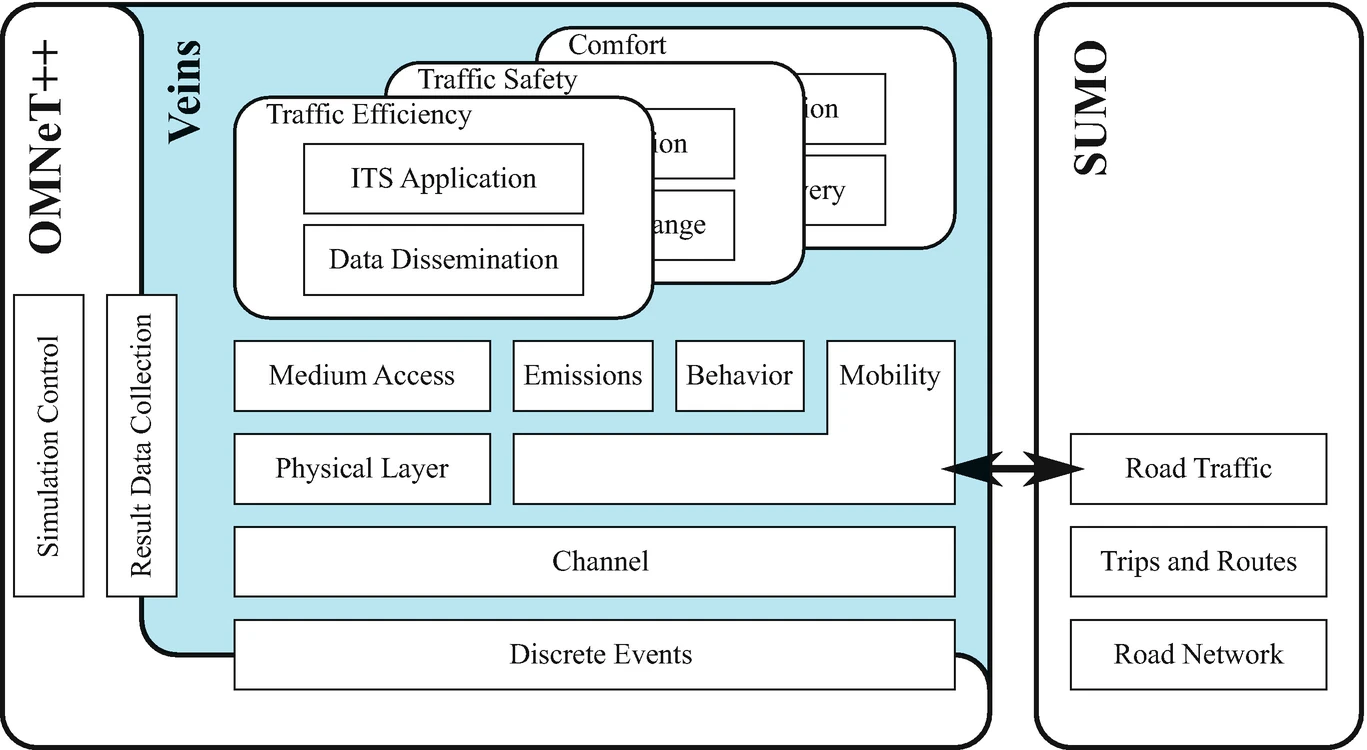
\includegraphics[width=1\textwidth]{figures/High-level Veins.png}
	\label{fig:veinshighlevel}
\end{figure}

\subsection{SUMO and TraCI}
As shown on \ref{fig:veinshighlevel}, Veins uses SUMO by \textcite[Page~218]{sumo2018} as a traffic simulator. According to the SUMO developers, SUMO is a microscopic traffic simulator, which means that each vehicle and its dynamics are modeled individually.
This a suitable solution for my scenario, because I indeed need each vehicle to be an independent object with its own known position. \cref{fig:sumogui} shows a screenshot of SUMO \ac{GUI}.

According to \textcite{traci}, \ac{TraCI} is a protocol, used to interlink road traffic and network simulators. The authors explain, that this protocol permits to control the behavior of vehicles during simulation time, therefore the network simulator can influence the driver's behavior. SUMO exposes \ac{TraCI} endpoints \cite{sumotraci} and Veins connects to them, allowing OMNeT++ user code to simulate \acp{VANET} \cite[Pages~217-218]{Sommer2019}. According to \textcite{Sommer2019}, Veins receives positions of vehicles from SUMO, these positions are later used as positions for network nodes, modeling vehicles in OMNeT++ simulation environment.

\begin{figure}
  	\caption{SUMO \ac{GUI} screenshot, gray rectangles depict obstacles (buildings), the black wide lines are the roads, the yellow triangle is a vehicle.}
	\centering
	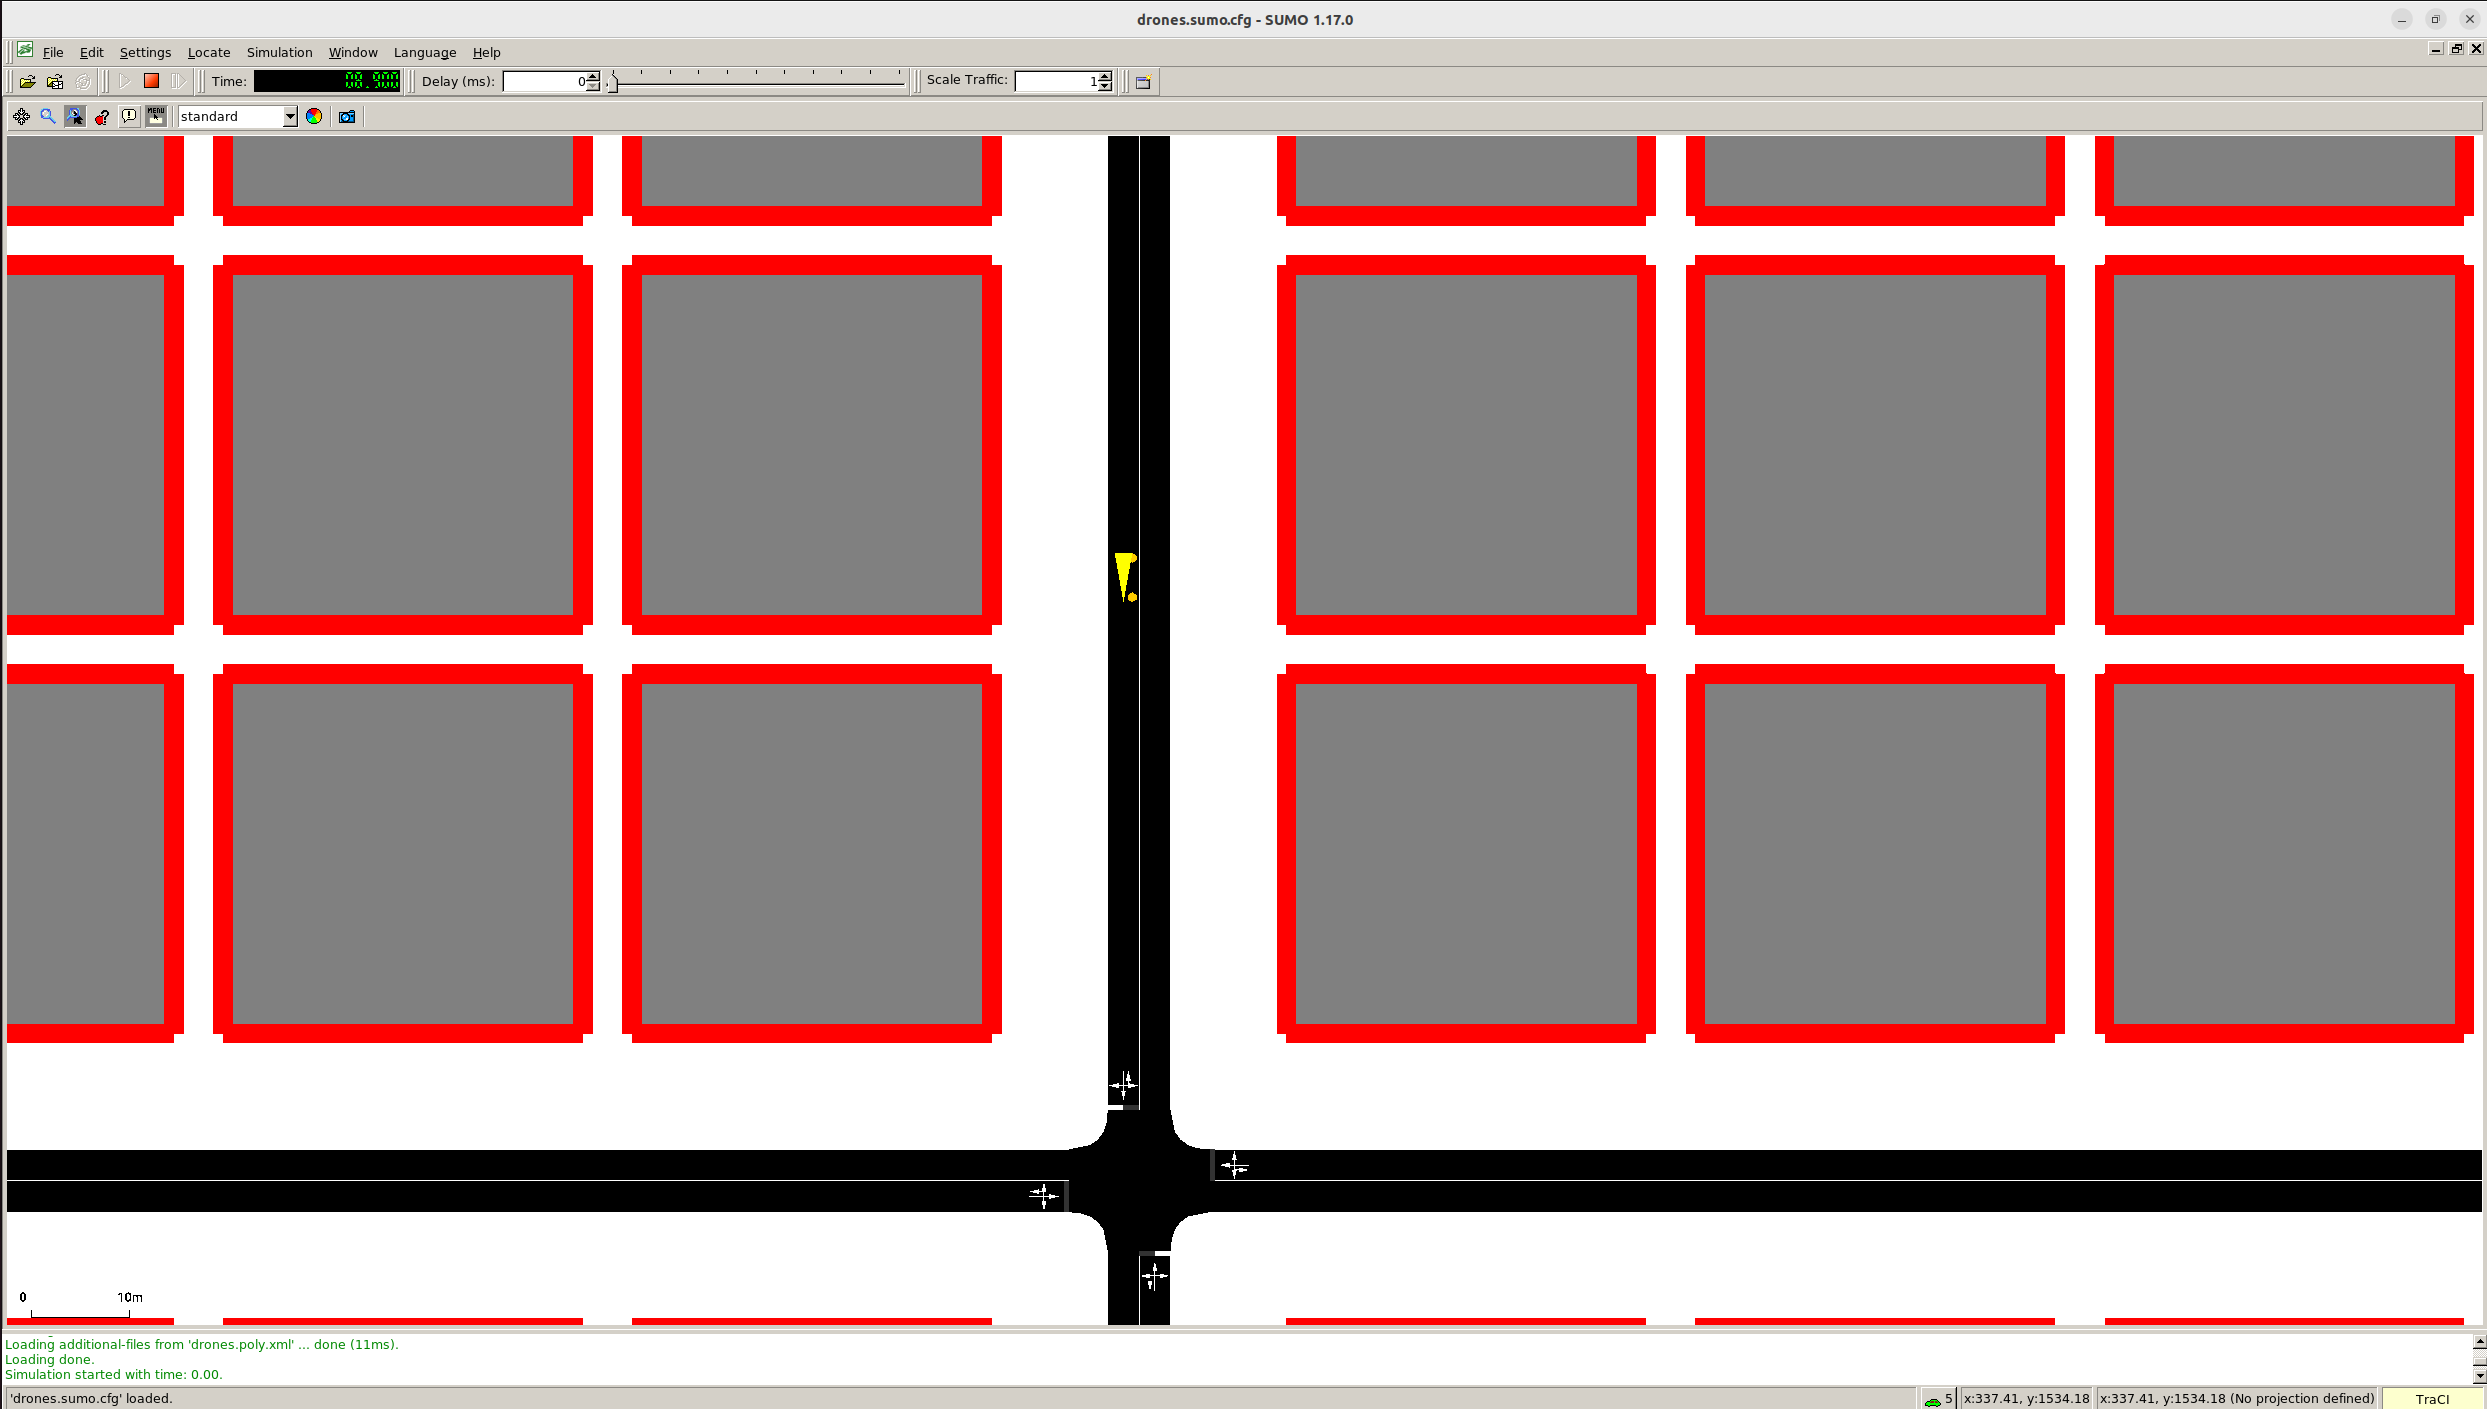
\includegraphics[width=1\textwidth]{figures/SUMO-GUI.png}
	\label{fig:sumogui}
\end{figure}

\subsection {Scenario and Car}
\label{sec:scenarioned}

To further understand my implementation of drones in Veins, it is necessary to consider two files included in Veins: the file Scenario.ned \cite{scenarioned} and the file Car.ned \cite{carned}. Scenario.ned defines the overall structure of the network, contains an array of all nodes and a list of auxiliary modules that control the vehicles or participate in the visualization when working with the GUI. The Car.ned file defines the structure of one of the most important modules - Car module, which is the internal representation of a vehicle. It contains, in particular, information about the network controller simulator and information about the user code of the application. Also, the Car module has a sub-module, which is responsible for synchronizing the movement with SUMO. Based on these two files in the future I will implement my version of the scenario, which will include drones in addition to vehicles, as well as support three-dimensional visualization of the scene. 

\begin{figure}
  	\caption{Simplified diagram of Scenario \cite{scenarioned} network. Not all modules, parameters and connections are shown.}
	\centering
	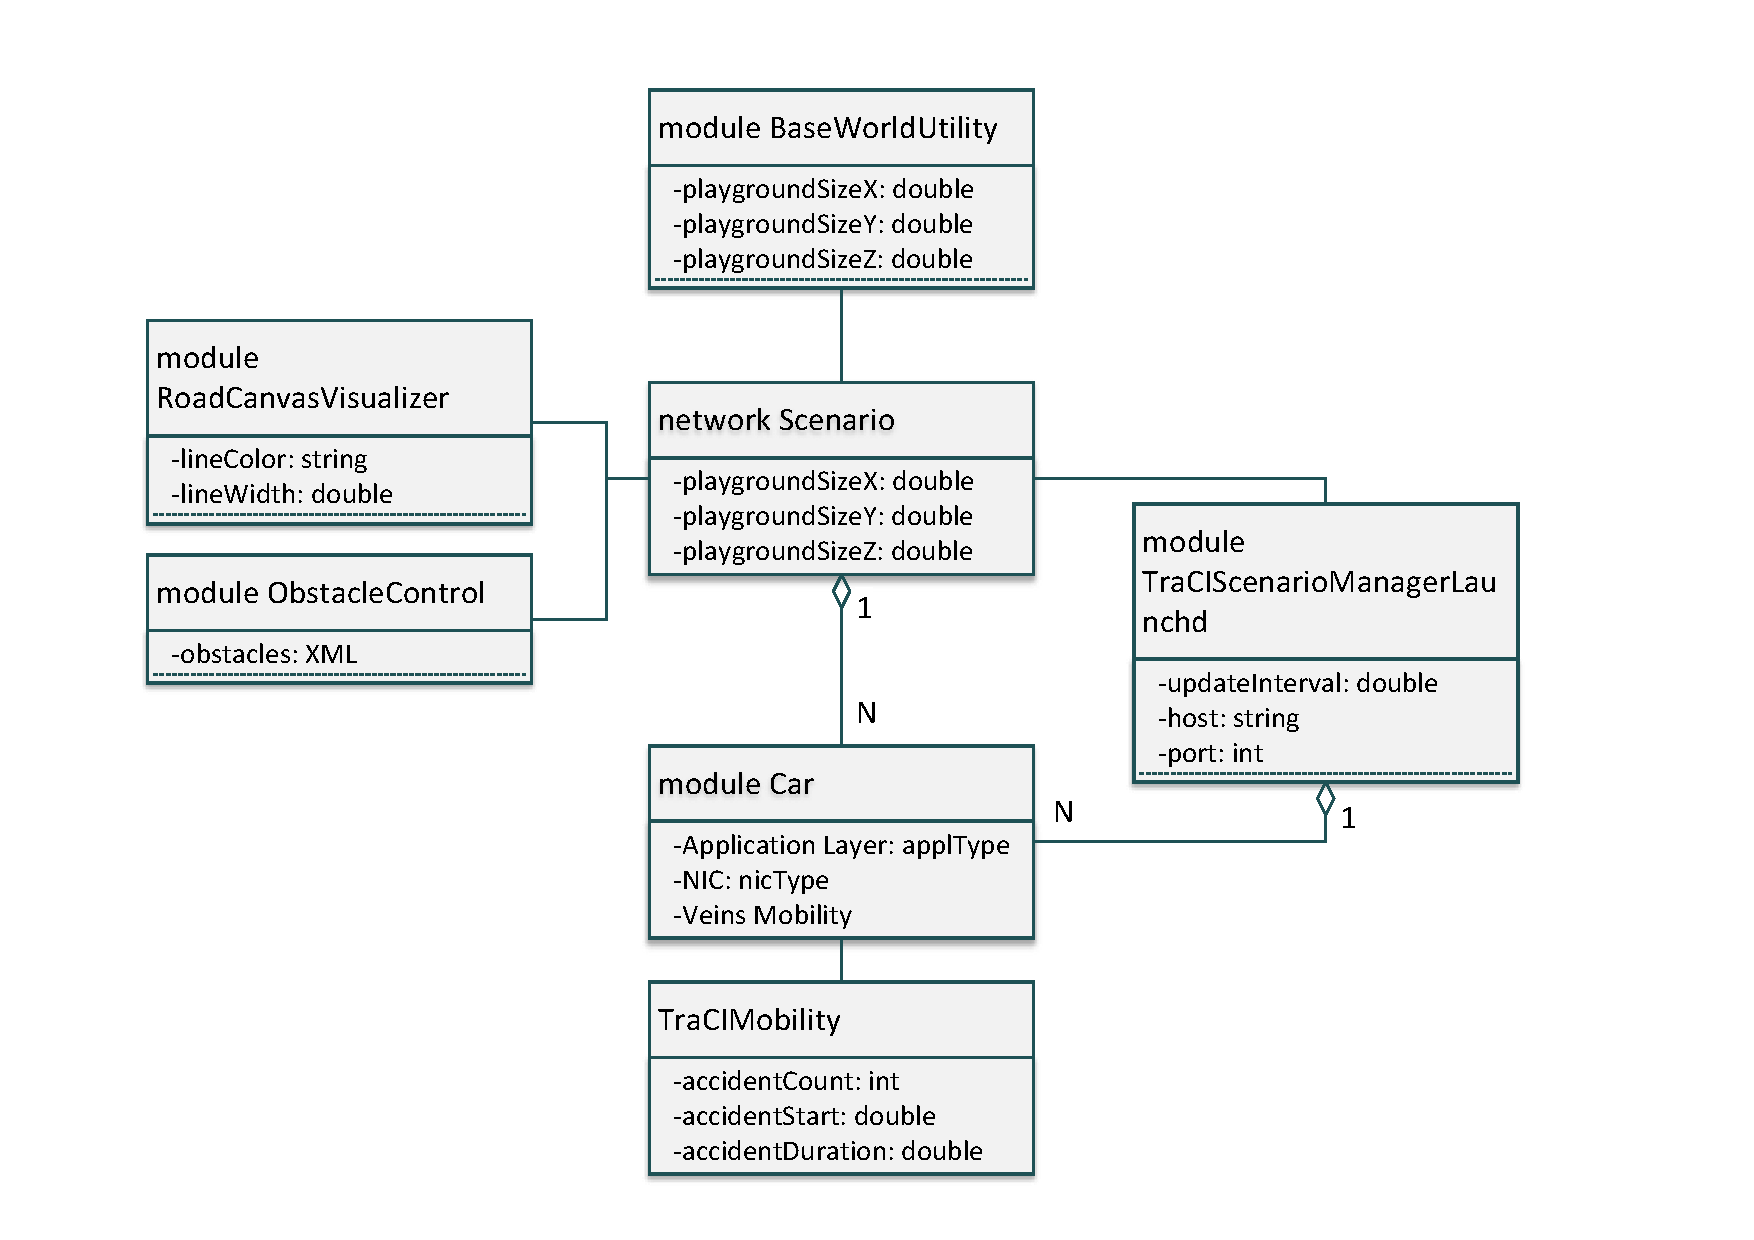
\includegraphics[width=1\textwidth]{figures/Scenario.pdf}
	\label{fig:scenarioned}
\end{figure}

\cref{fig:scenarioned} shows a simplified diagram of the network in Veins. It is not a diagram of classes in the usual sense, it shows the relationship of OMNeT++-modules and OMNeT++-networks , as well as some parameters that will be of interest in the rest of the work. 

\subsection{2D Simple Shadowing}

Next in my work I will describe the algorithm that calculates the fading of the radio signal, which takes into account three-dimensional objects. My algorithm is based on the Simple Obstacle Shadowing algorithm \cite{SimpleObstacleShadowing} that is implemented in Veins, and therefore I will briefly describe it here. In Veins' Simple Obstacle Shadowing algorithm each building is defined as a 2D-polygon with arbitrary number of vertices. The radio transmission is modeled as a ray starting from sender's antenna and ending in receiver's antenna. The algorithm determines, how much of the total distance the radio signal traveled through a building. Based on this information the algorithm than calculates the power with which the radio signal reaches the receiver. The signal can penetrate an arbitrary number of buildings. The algorithm also allows the user to set values that determine, how much buildings block the signal via their walls and via their interior. A graphical representation of this model can be seen on \cref{fig:SimpleObstacleShadowing}

\begin{figure}
  	\caption{Visualization of the Simple Obstacle Shadowing algorithm implemented in Veins. The gray rectangles depict buildings (or any other obstacles), white circles are the points of intersection between radio signal and obstacles' walls.}
	\centering
	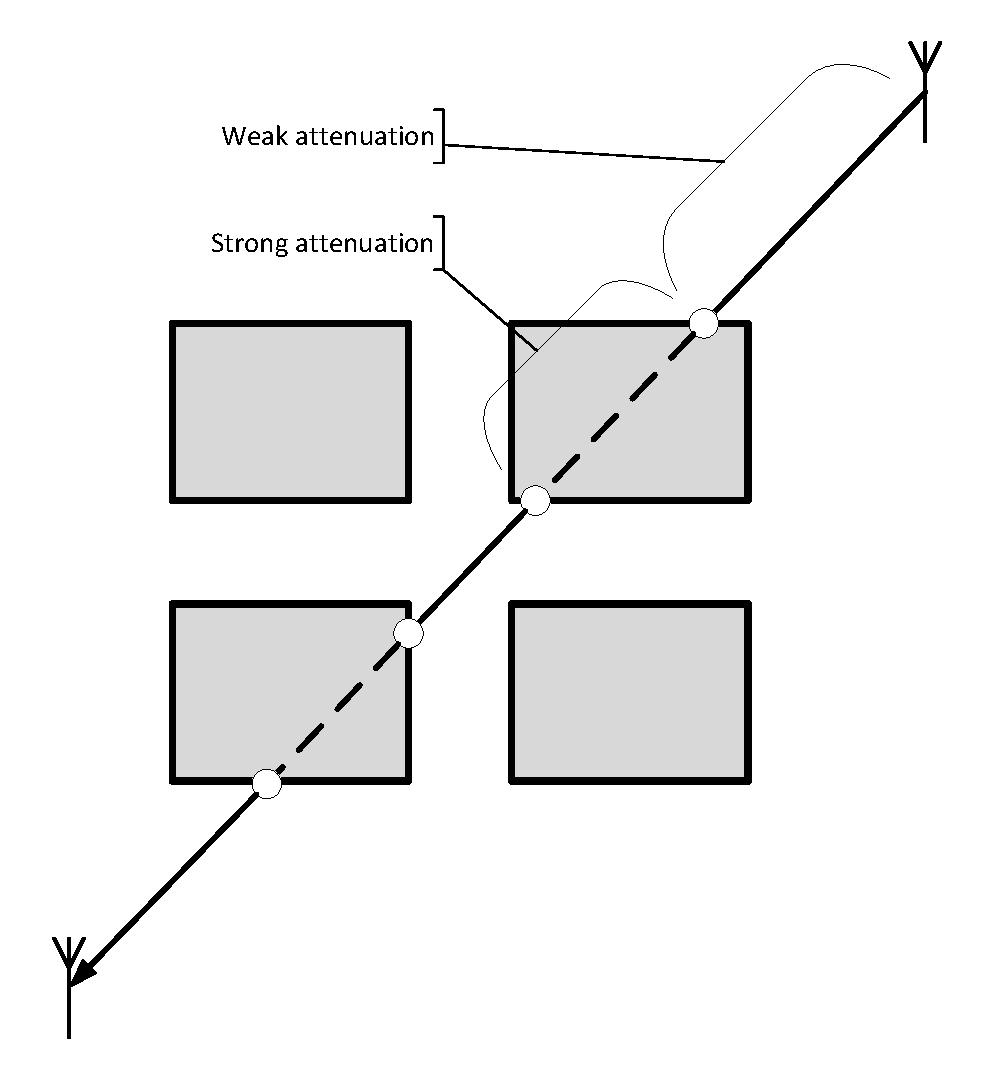
\includegraphics[width=1\textwidth]{figures/SimpleObstacleShadowing.pdf}
	\label{fig:SimpleObstacleShadowing}
\end{figure}

\subsection{OpenSceneGraph}

I would like to emphasize the usage of OpenSceneGraph \cite{osg} as a 3D-rendering tool.  OMNeT++ natively supports OpenSceneGraph \cite{omnetpposg}, therefore \ac{OSG} is the most convenient and easy way to implement a 3D scene in OMNeT++. In this work, I will use 3D visualization for debugging purposes.

Veins provides a C++ class for \ac{OSG}-based road visualization. I will utilize this class along with my own vehicle-, drone- and building- visualizers.

\subsection{IEEE 802.11p}
Veins includes a simple simulation model of IEEE 802.11p for vehicle-to-vehicle communication \cite[Page~216]{Sommer2019}. The following brief description of IEEE 802.11p is based on \textcite{IEEE80211p}.

IEEE 802.11p is a set of standards dedicated exclusively to vehicle-to-vehicle and infrastructure-to-vehicle communication. It uses 75 MHz of \ac{DSRC} spectrum at 5.9 GHz. The primary goal is to enable public safety applications that can help with road safety and improve traffic flow. Private services are permitted to use these frequencies. The \ac{DSRC} band is free, but licensed spectrum, therefore it is more restricted in terms of usages and technologies in comparison to unlicensed spectrums like Wi-Fi. \ac{DSRC} can be used only for vehicular networks, nobody is allowed to develop another technology, that uses the same radio spectrum. The key feature of IEEE 802.11p is the WAVE mode, that allows a vehicles to communicate immediately upon encounter, without the overhead of scanning for channels and executing handshakes. 

In my work I will use Veins-provided IEEE 802.11p simulation model for both vehicles and drones, working in WAVE mode.

\chapter{Implementation}

Now it is time to develop a network model for a scenario in which vehicles and drones will interact within the same virtual space. My implementation is largely based on the model used in Veins, which was discussed in \cref{sec:scenarioned}. My model basically repeats the structure of the model from Veins, as the basic modules remain the same. However, I have integrated into my model drones, support for the third dimension when calculating sight lines, and special modules for using OSG to render a three-dimensional scene. A schematic view on the communication between drones and vehicles can be seen on \cref{fig:vanetscheme}. \cref{fig:dronescenarioned} shows a simplified UML diagram of classes for the OMNeT++ network in my model, the scheme is analogues to \cref{fig:scenarioned} and is meant to show similarities and differences between my model and Veins' model.

\FIXME{VANET scheme.png - Drone image is not mine!}

\begin{figure}
  	\caption{Schematic view on the network. My scenario does not include any infrastructure, the \ac{V2V}, \ac{V2D} and \ac{D2D} communication is implemented using the same IEEE 802.11p model, provided by Veins.}
	\centering
	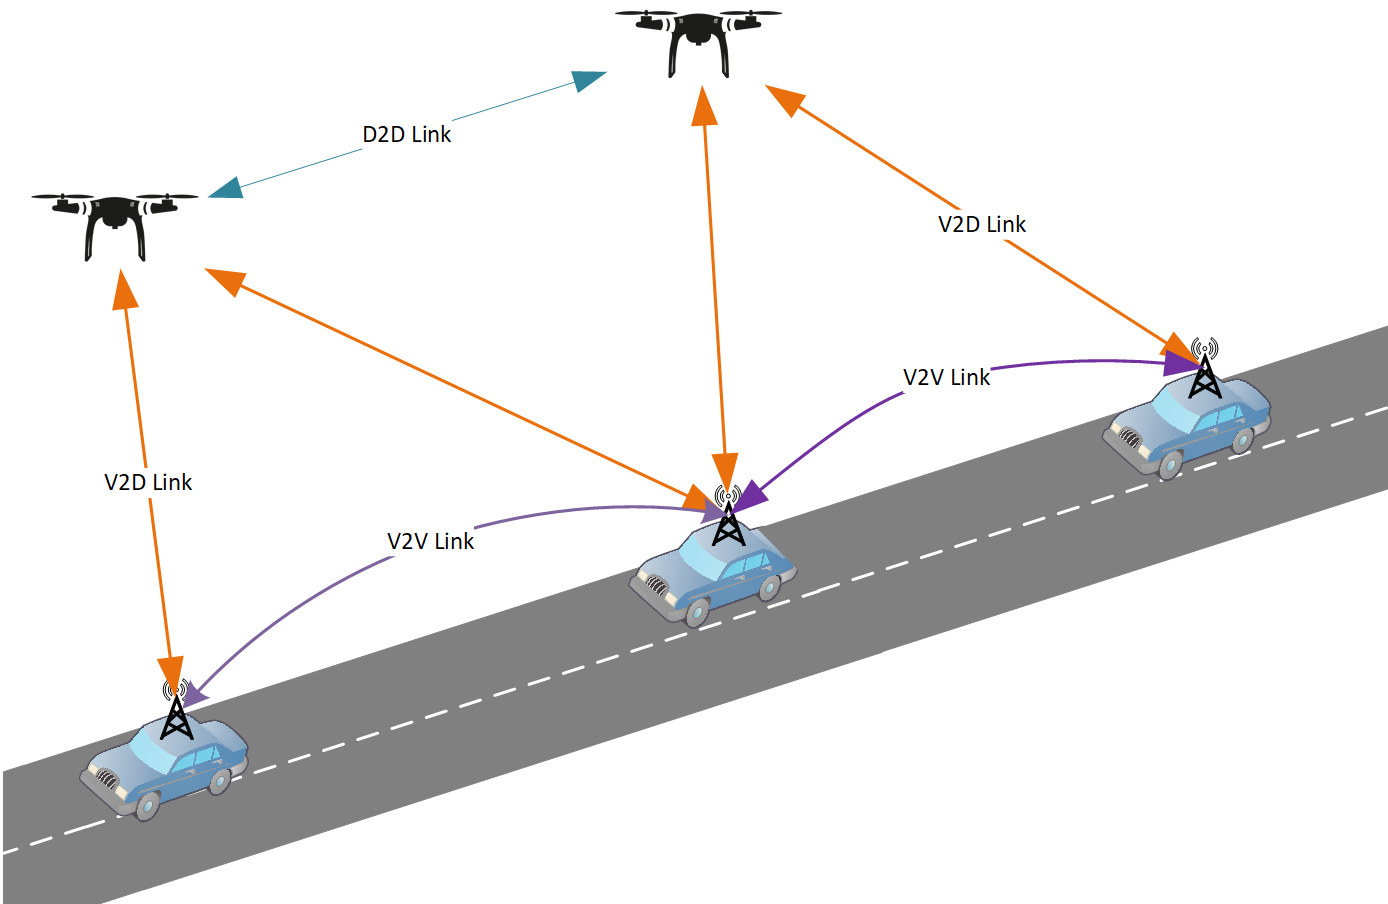
\includegraphics[width=1\textwidth]{figures/VANET scheme.png}
	\label{fig:vanetscheme}
\end{figure}

\begin{figure}
  	\caption{Simplified diagram of DroneScenario network. In contrast to Veins, the following modules were added to the network: ObstacleShadowingVisualizer, Pathfinder, DroneManager and array of Drones. Some modules replace analogues Veins modules to add new functionality: RoadsOsgVisualizer2, ObstacleControl3d, array of Car3d}
	\centering
	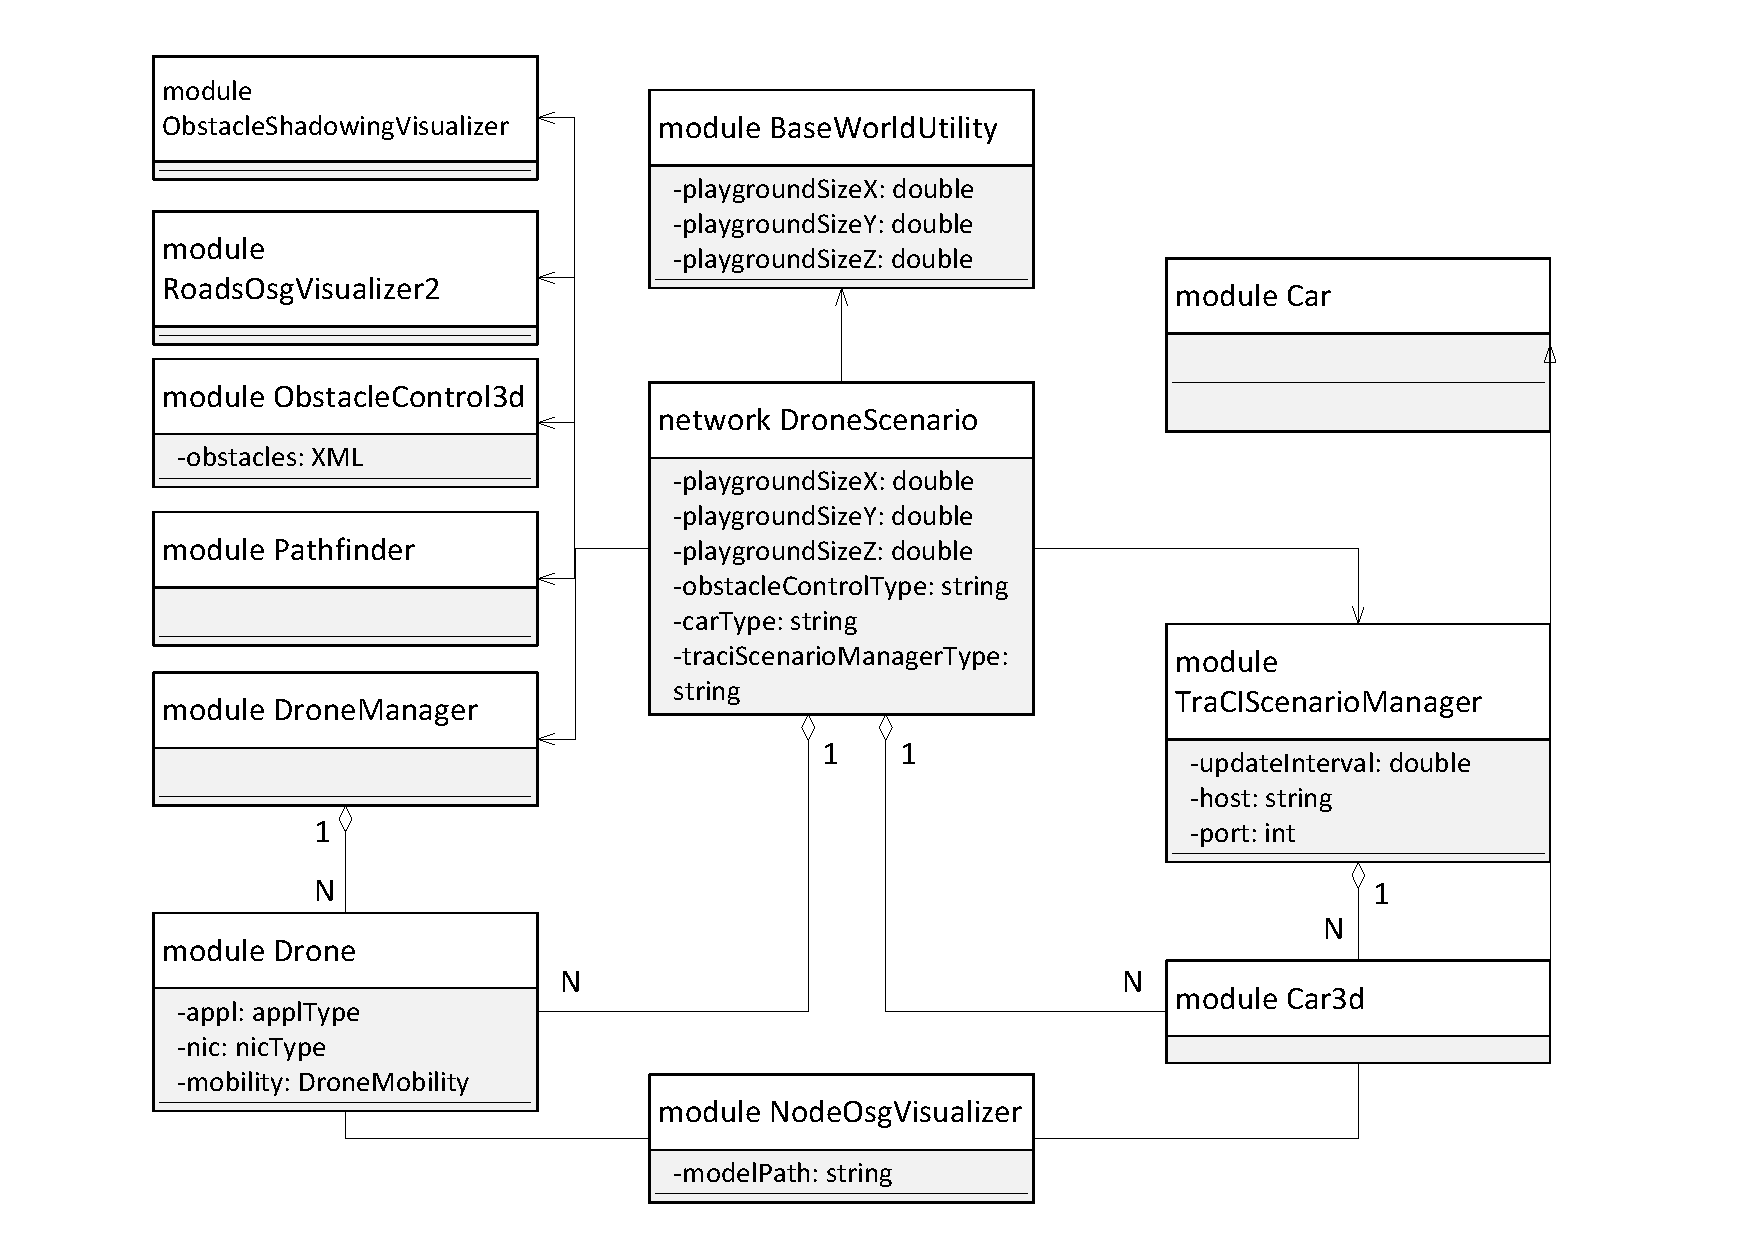
\includegraphics[width=1\textwidth]{figures/DroneScenario.pdf}
	\label{fig:dronescenarioned}
\end{figure}

\section{Drones}

The first issue with implementing my scenario is that Veins does not support drones. Therefore, implementing drones was on of the first steps in my work. The easiest way to implement drones would be to reuse the existing Veins' code, that was used for vehicles. Therefore, drones will in fact only differ in their mobility, but in other things they will mostly share the code with Veins' vehicles.

\cref{fig:dronened} shows a simplified structure of the Drone.ned module. Like the Car.ned from Veins, Drone.ned uses a special submodule for moving in space. To improve simulation efficiency (i.e., to reduce the number of events), all drone movements are performed once every 1 second as part of the single event processing. The DroneManager.ned module is responsible for managing this event (scheduling and execution), as well as for creating and removing drones. Simply put, the DroneManager module creates a specified number of drones, and then sends a position update signal to each drone at a period of 1 second (configurable). 

\begin{figure}
  	\caption{Simplified diagram of Drone module.}
	\centering
	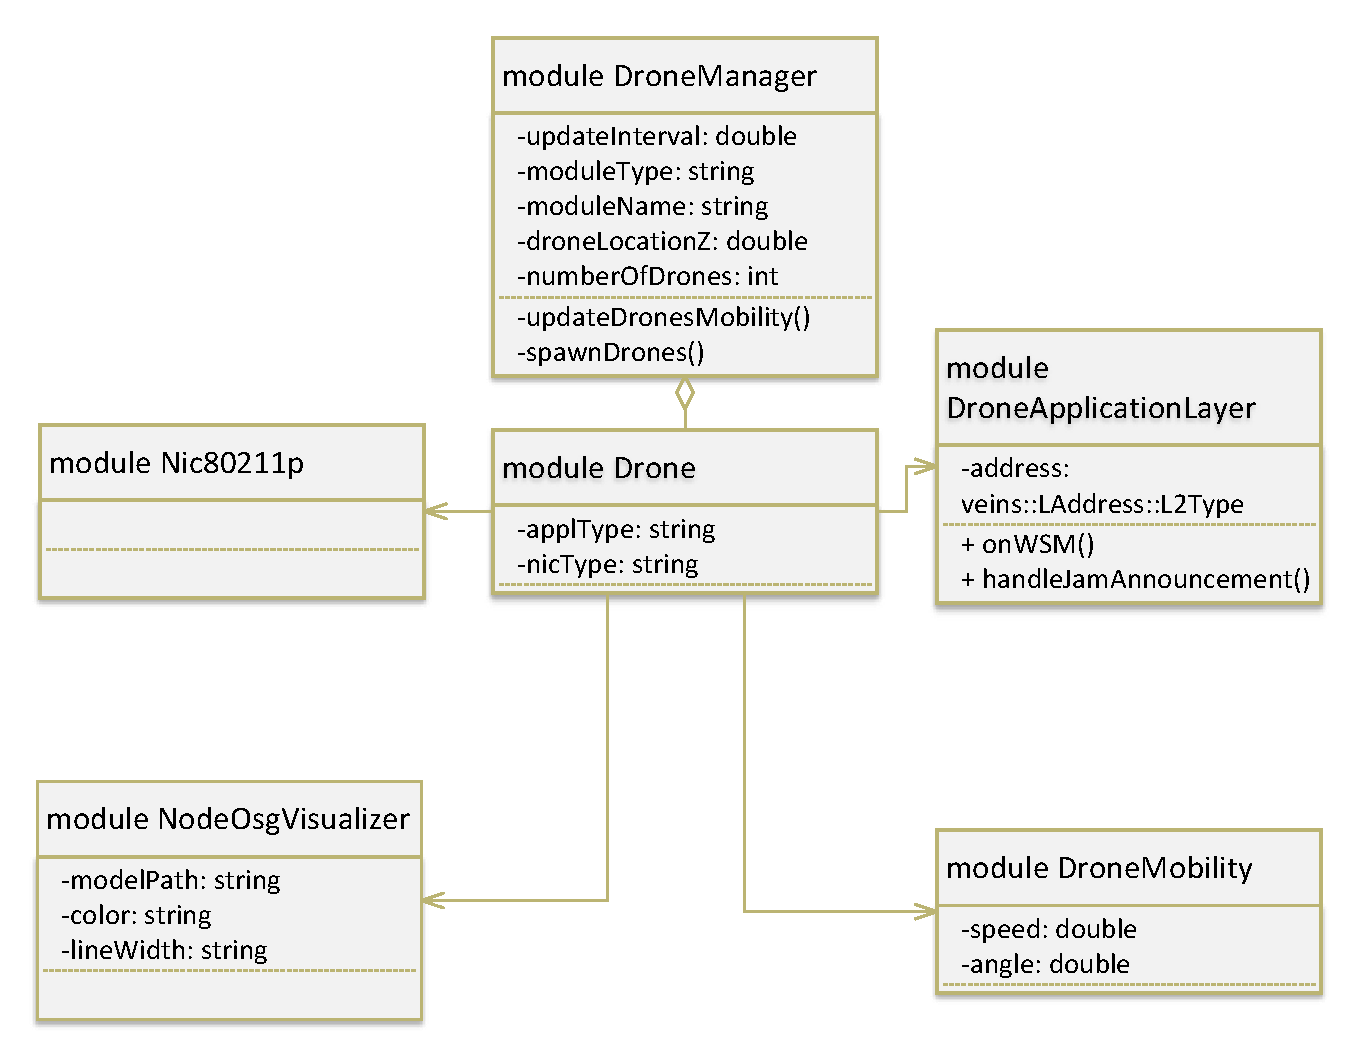
\includegraphics[width=1\textwidth]{figures/Drone.pdf}
	\label{fig:dronened}
\end{figure}

\subsection{Drone Mobility}

DroneMobility submodule is based on Veins' LinearMobility with some minor changes. The biggest one: DroneMobility does not update itself. Instead, the DroneManager calls a special method that makes DroneMobility to update its position.

The \cref{fig:dronemanagerflow} shows a simplified algorithm for updating the drone's position. The drones themselves use the methods implemented in Veins to update their position. The Z-coordinate of each drone can be set through a configuration file.

\begin{figure}
  	\caption{Simplified flowchart of DroneManager updating DroneMobility submodules of each Drone.}
	\centering
	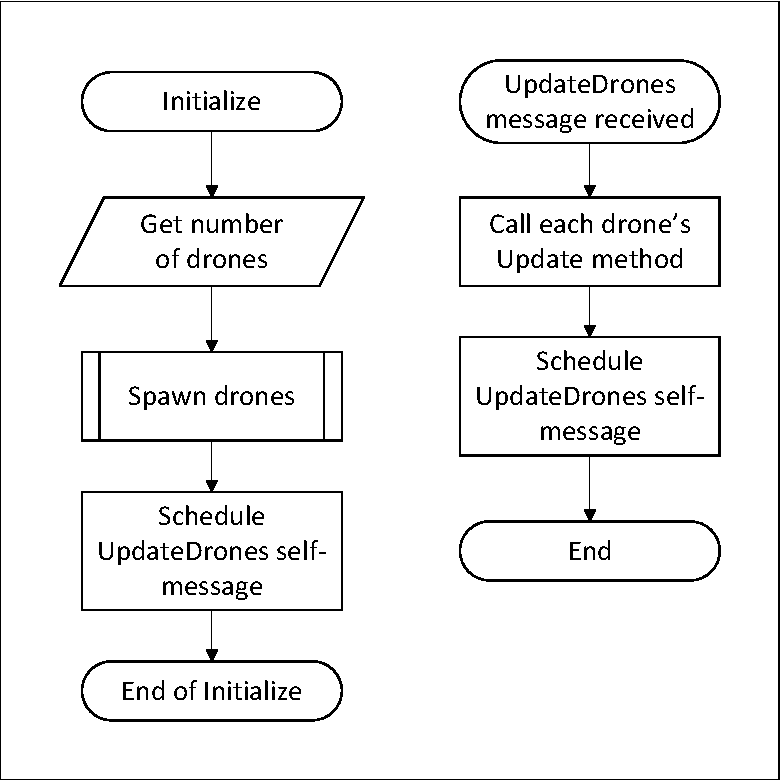
\includegraphics[width=1\textwidth]{figures/DroneManager.pdf}
	\label{fig:dronemanagerflow}
\end{figure}


\section{BaseApplicationLayer}

To integrate the drones more easily, I decided to create an additional level of abstraction: BaseApplicationLayer (\cref{fig:baseapplicationlayer}), which will be common for drones and cars. This class is responsible for automatically assigning network addresses, for keeping track of statistics common to drones and cars, and, importantly, for decisions about relaying incoming messages. BaseApplicationLayer inherits from DemoBaseApplLayer, that is implemented in Veins.

\begin{figure}
  	\caption{Simplified diagram of BaseApplicationLayer. Not all parameters are shown. DemoBaseApplLayer is implemented in Veins \cite{demobaseappllayer}}
	\centering
	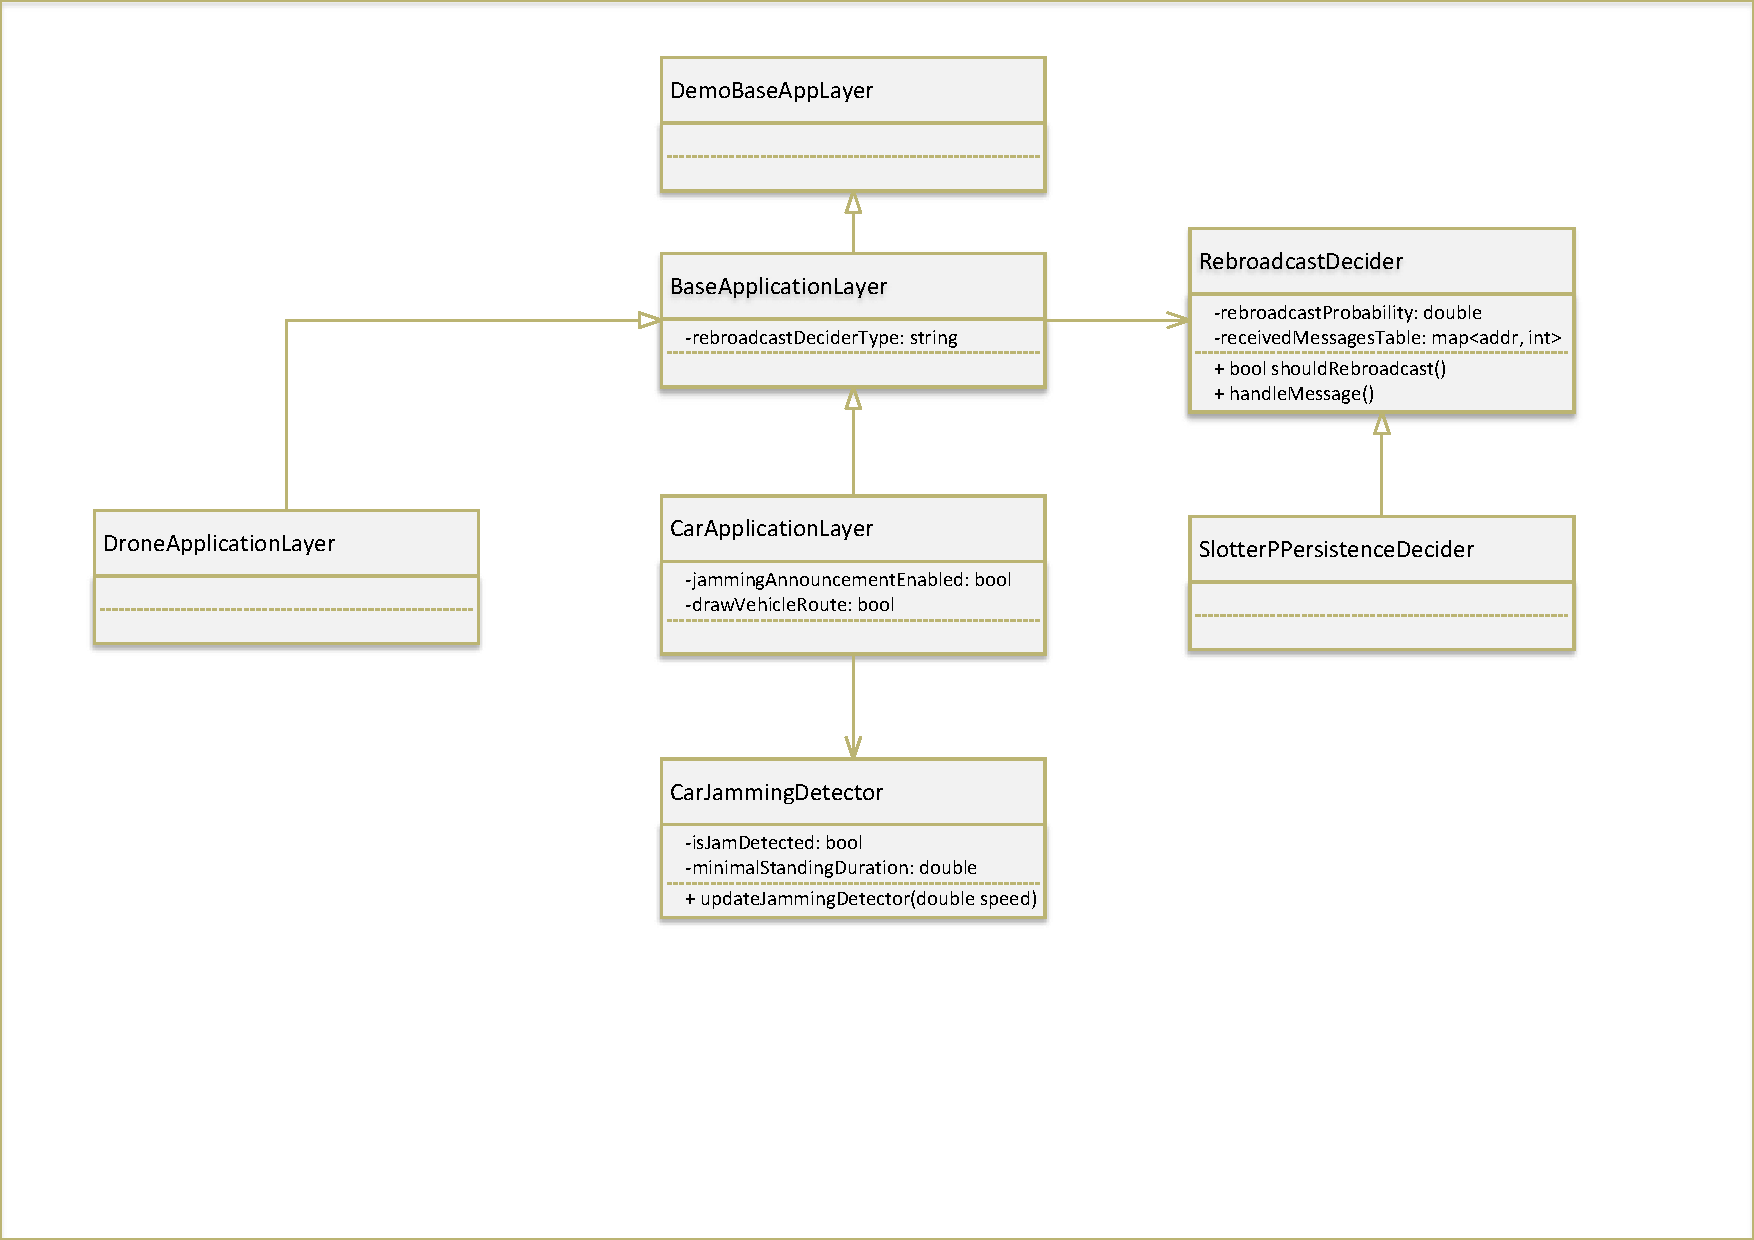
\includegraphics[width=1\textwidth]{figures/BaseApplicationLayer.pdf}
	\label{fig:baseapplicationlayer}
\end{figure}

The main reason for creating the BaseApplicationLayer is to unify the way how decision about rebroadcasting is made. BaseApplicationLayer holds a reference to a special object of class RebroadcastDecider, which in fact is a virtual class. This object decides whether to rebroadcast the message or not. How exactly it makes this decision for the vehicle or for the drone is irrelevant. The drone or vehicle only receives a decision from this object. So it is relatively easy to change the algorithm that decides whether to retransmit a message. Also it is easy to enable a specific algorithm for both drones and vehicles in the same manner.

\subsection {Rebroadcast Decider}

As you can see in \cref{fig:baseapplicationlayer}, BaseApplicationLayer is associated with an object of the RebroadcastDecider class, which is also an OMNeT++ module. Objects of this class are responsible for rebroadcasting packets. The point of providing a separate object is that both drones and cars can use different interchangeable broadcast storm suppression algorithms. 

The \cref{fig:rebroadcastdeciderseq} shows the sequence of message exchange between the broadcast medium and network nodes (drone or vehicle). In some places, the activation time of the actor is not shown. This is done to indicate that at these points in the sequence the packet processing time is zero in terms of simulation time. Packets reach the RebroadcastDecider instantaneously as soon as they have been received and decoded. It should also be noted that in case the RebroadcastDecider decides to rebroadcast a packet, this can happen at any point in time and any number of times (depending on the particular implementation of the RebroadcastDecider).

\begin{figure}
  	\caption{UML Sequence for RebroadcastDecider. Note that other messages, unrelated to RebroadcastDecider are not shown.}
	\centering
	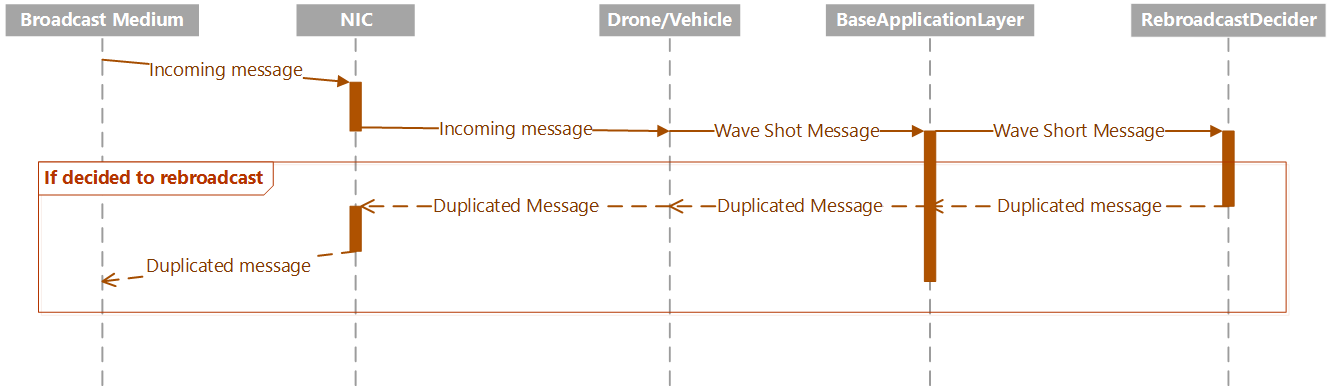
\includegraphics[width=1\textwidth]{figures/RebroadcastDecider.png}
	\label{fig:rebroadcastdeciderseq}
\end{figure}

\section{Adding the third dimension}

The next problem was that Veins does not support three-dimensional obstacles, and therefore does not take Z coordinate into account when calculating radio signal decay. In my scenario, this is a significant drawback, since drones tend to fly above buildings, and hence their radio transmissions are not affected by buildings. In that case, one could make the radio transmissions between drones simply ignore the buildings. However, such a strategy would ignore radio signals between drones and cars. Drone-vehicle communication cannot be described by simple rules from 2D space with at least acceptable accuracy. Because of this, I decided to implement three-dimensional buildings and, accordingly, a three-dimensional algorithm for signal shadowing.

\subsection{3D buildings and signal shadowing}

In my work I assume that buildings can be approximated as right prisms, example shown in \cref{fig:rightprism}. 

\begin{figure}
  	\caption{Example of a right prism. The bases are two equal arbitrary polygons, and the walls are rectangles with equal height perpendicular to the bases. The right prism can be easily imagined via "extruding" a random polygon straight upwards.}
	\centering
	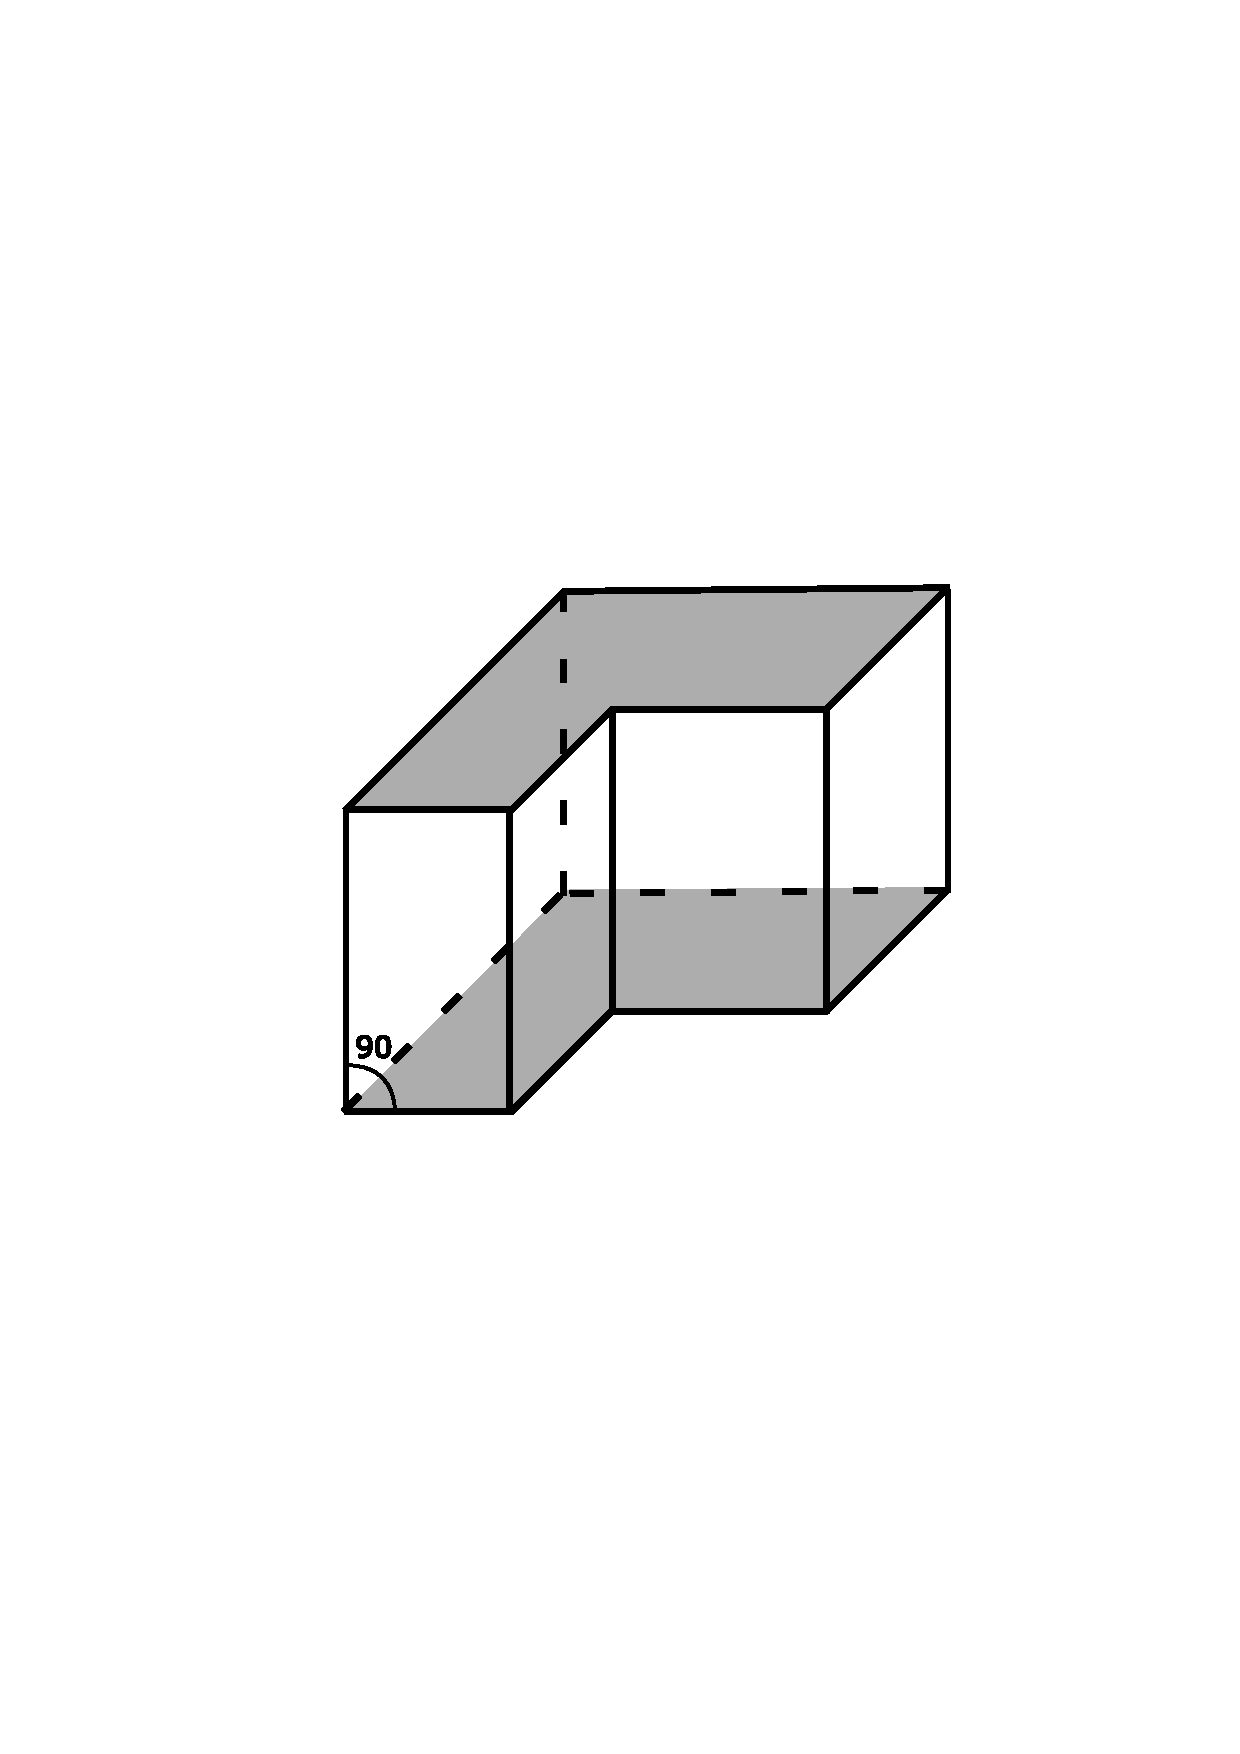
\includegraphics[width=1\textwidth]{figures/RightPrism.pdf}
	\label{fig:rightprism}
\end{figure}

This way a 3D shadowing algorithm can be extended from Veins' Simple Obstacle Shadowing. Instead of looking for intersections of 2D rays with 2D polygons, I will look for intersections of 3D rays with right prisms. The classes, used to augment the Veins' code are shown on \cref{fig:obstacle3d-classes}.  Basically, my class ObstacleControl3d reuses Veins' ObstacleControl and only overrides some methods in order to spawn Obstacle3d objects instead of Veins' Obstacle objects. Also ObstacleControl3d reads obstacles' height from the same xml file, that Veins uses, but additionally reads the \emph{height} attribute to set Obstacle3d's height. If this attribute is not found, ObstacleControl3d uses its configuration parameter to set the default height for obstacles. The search for intersections is done inside Obstacle3d. This class inherits Vein's Obstacle class, but adds new methods that calculate line-right-prism intersection. The simplified flow chart of Obstacle3d's algorithm can be seen on \cref{fig:obstacle3d-flow}. 

\begin{figure}
  	\caption{Simplified diagram of classes for 3D obstacles system.}
	\centering
	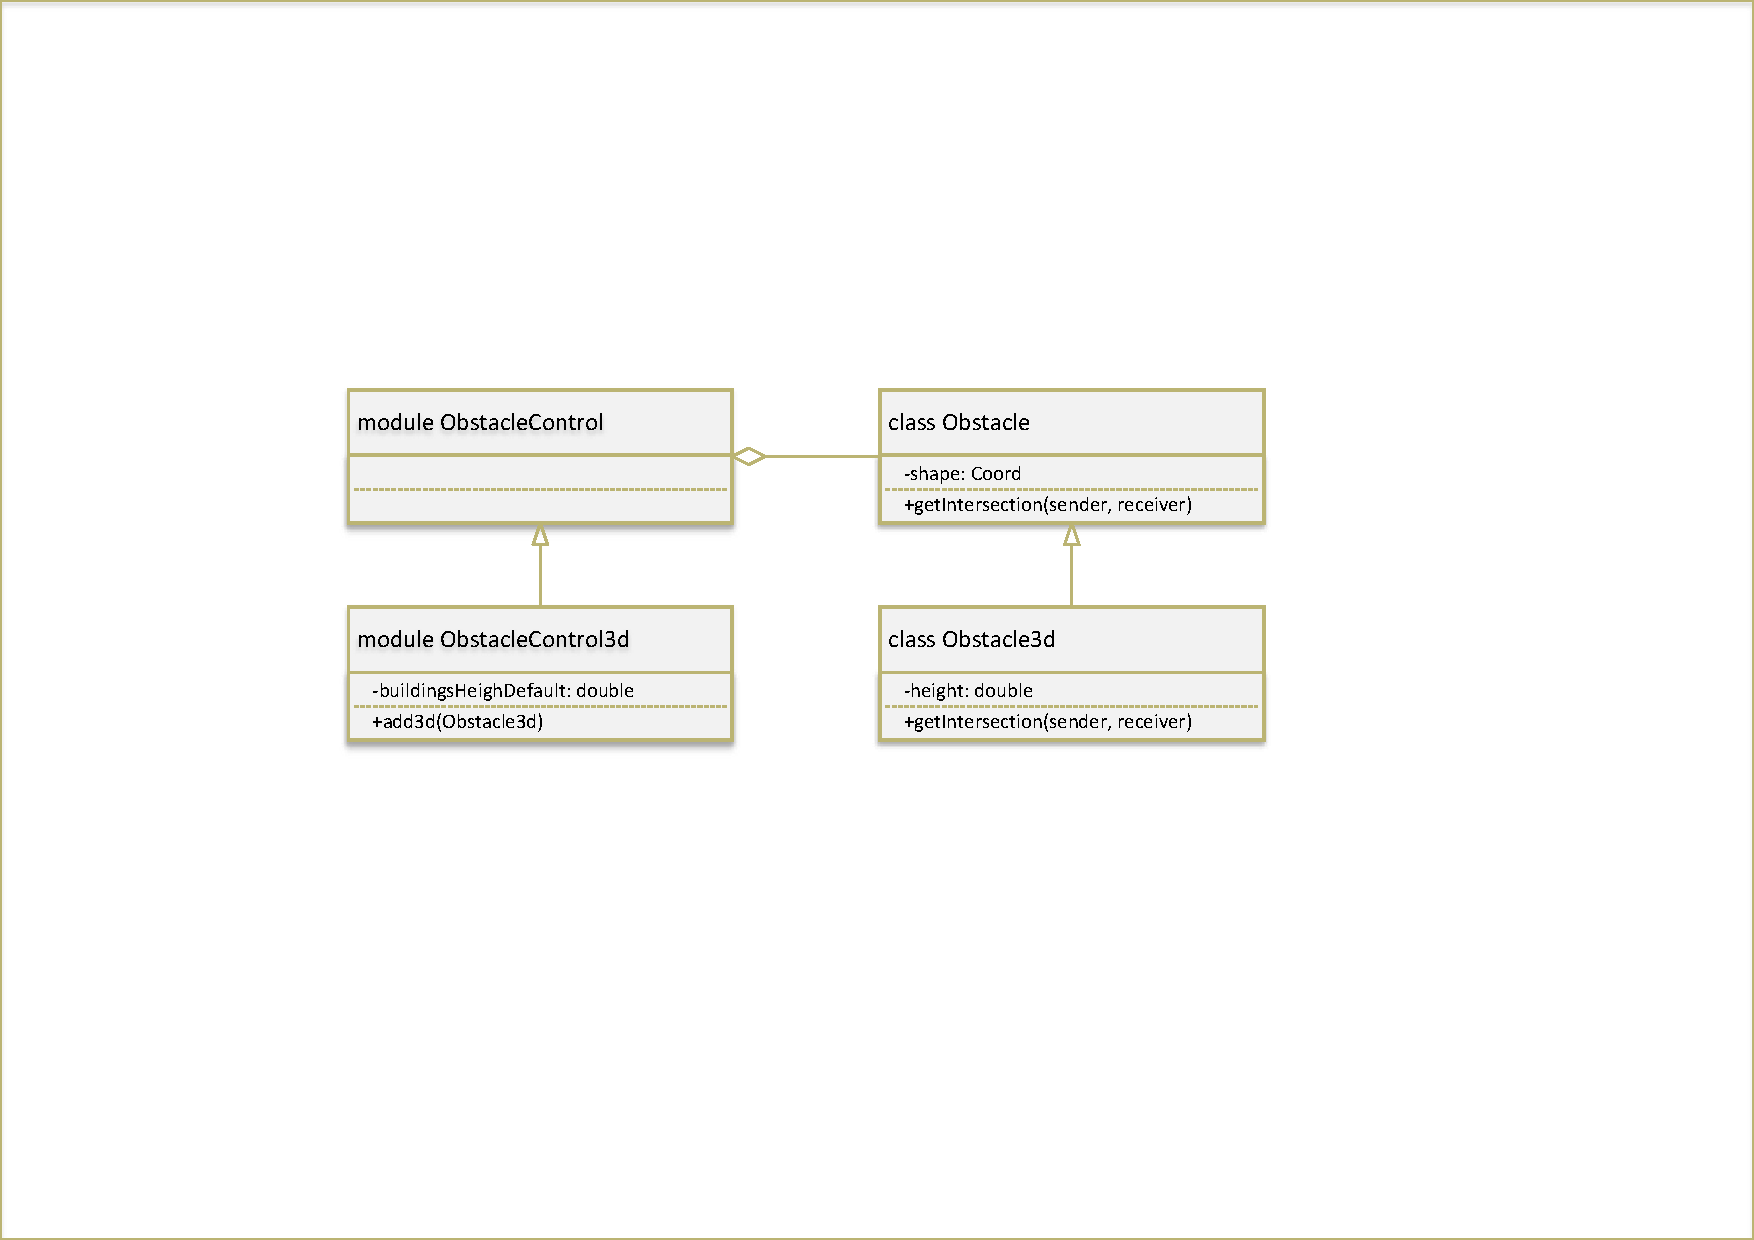
\includegraphics[width=1\textwidth]{figures/Obstacle3d-classes.pdf}
	\label{fig:obstacle3d-classes}
\end{figure}

\begin{figure}
  	\caption{Flowchart of line-right-prism intersection algorithm. Flow for only single Obstacle3d is shown. The ObstacleControl3d iterates over all Obstacle3d objects, calls their getIntersections() methods and combines results.}
	\centering
	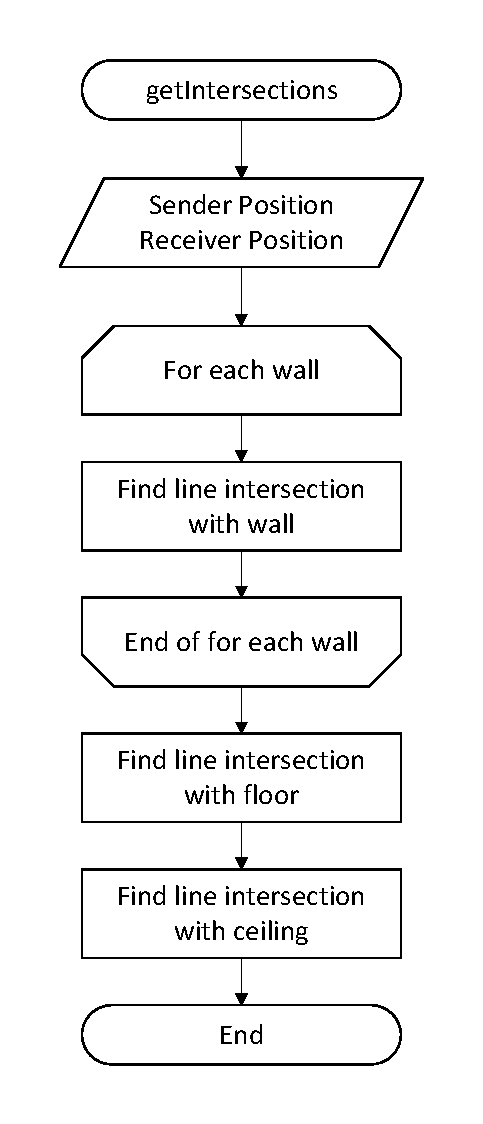
\includegraphics[width=1\textwidth]{figures/Obstacle3d-flow.pdf}
	\label{fig:obstacle3d-flow}
\end{figure}

\subsection{3D visualization}

Developing with algorithms that work with 3D objects becomes very complicated without a possibility of visual debugging. In order to easily debug the simulation I have decided to implement 3D visualization of the virtual environment, including vehicles, drones, and buildings. OMNeT++ supports OpenSceneGraph as a 3D rendering library, and my solution also uses it. 

The central modules that are responsible for 3D visualization in my project are: 

\begin{itemize}

\item \textbf{NodeOsgVisualizer} - provided with a file path to a 3D model, draws this model on the \ac{OSG} canvas using the parent's position. Also utilizes Vehicle's heading angle. 

\item \textbf{Obstacle3d} - in addition to methods for finding intersections with a prism, also draws a prism on the \ac{OSG} canvas.

\item \textbf{ObstacleShadowingVisualizer} - draws radio transmission as 3D lines on the \ac{OSG} canvas. Also shows intersections with 3D obstacles. 

\end{itemize}

\begin{figure}%
    \centering
    \subfloat[Vehicle]{\label{fig:vehicle-model}\includegraphics[width=0.5\textwidth]{figures/car3d-model.png}}%
    \subfloat[Drone]{\label{fig:drone-model}\includegraphics[width=0.5\textwidth]{figures/drone-model.png}}
    \caption{3D models created for the project. 3D visualizations of buildings are generated at runtime.}%
    \label{fig:3dmodels}%
\end{figure}

\begin{figure}
  	\caption{ObstacleShadowingVisualizer work example. Radio signals are emitted from the vehicle and are shown as blue lines. Red spheres depict intersections with buildings. Note that the drone and the vehicle are not in scale, they are intentionally made visually bigger in order to make them visible. Model scale can be adjusted in configuration file.}
	\centering
	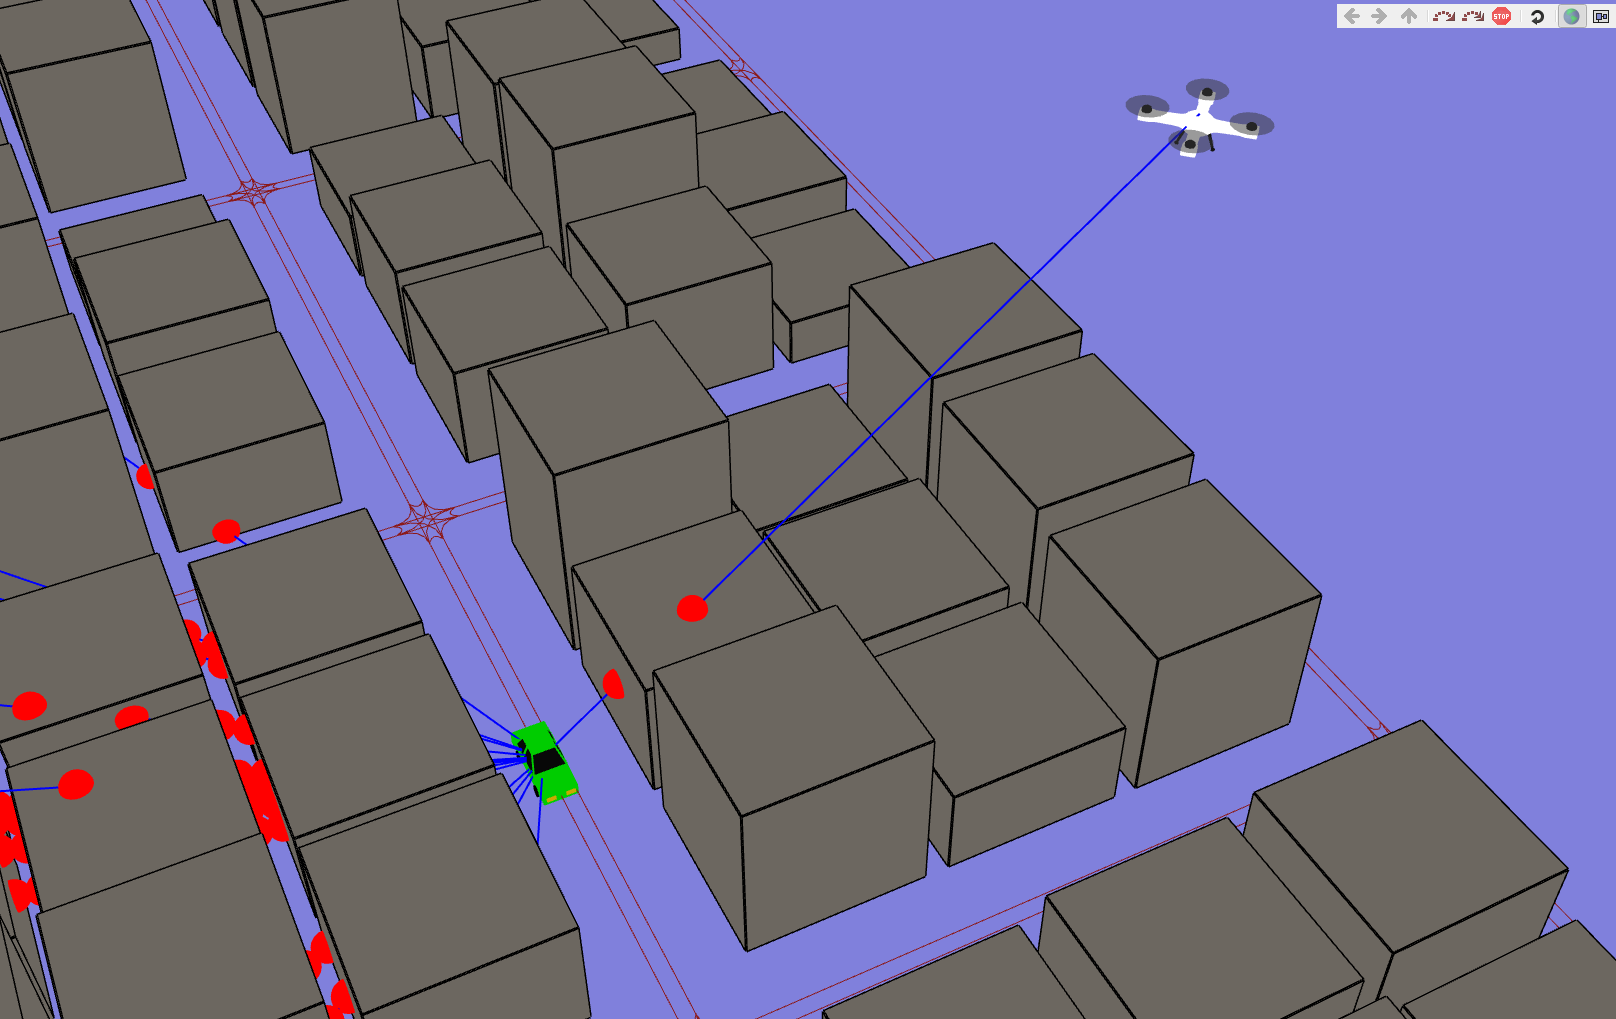
\includegraphics[width=1\textwidth]{figures/ObstacleShadowingVisualizer.png}
	\label{fig:ObstacleShadowingVisualizer}
\end{figure}


\section{Protocol}

Finally, I will explain the protocol that is used in communication between vehicles and drones. The protocol is based on IEEE 802.11p, a simulation of which is implemented in Veins. 

In my project, a single broadcast message is defined, which the cars send to the air in case of an unforeseen stop. This message is called CarJammingAnnouncement and it contains the following information:

\begin{itemize}

\item \textbf{Sender Address} - integer field, representing a unique address of a network node. The jammed vehicle sets this field to its address upon initial broadcast.

\item \textbf{Serial} - integer field, monotonically increasing counter locally handled by each vehicle. Together with Sender Address makes sure, that each CarJammingAnnouncement is unique.

\item \textbf{Car Road Id} - SUMO id of a road, on which the vehicle is jammed. Its real-life equivalent can be name of a street.

\item \textbf{Car Position} - OMNeT++ coordinates on which the vehicle is jammed. This field's real-life equivalent can be GPS coordinates.

\item \textbf{Sender Timestamp} - time of broadcast. Used to calculate latency.

\item \textbf{Last Rebroadcaster Position} - OMNeT++ coordinate of last node (drone or vehicle) that rebroadcast this message. While the Car Position is always the position of a jammed vehicle, that originally sent the message, the Last Rebroadcaster Position depends on the context of the rebroadcast.

\end{itemize}

\cref{fig:protocol} shows how the CarJammingAnnouncement is propagated through the network. The protocol is based on the distribution of broadcast messages about the occurrence of a traffic jam. When a message is received, the vehicle checks if its route goes through the road whose identifier is contained in the message. If it does, the vehicle remembers this identifier (makes a list of all roads where a traffic jam occurred) and recreates the route so that it does not get into the traffic jam. After receiving the message, the vehicle sends the message back on the air according to the rules for avoiding broadcast storms. Drones act in the same way, except that they ignore the information about the traffic jam in the message. They only rebroadcast a copy of the message.

\FIXME{\cref{fig:protocol} does not fit!}

\begin{figure}%
	\centering
	\subfloat[Step 1]{\label{fig:protocol1}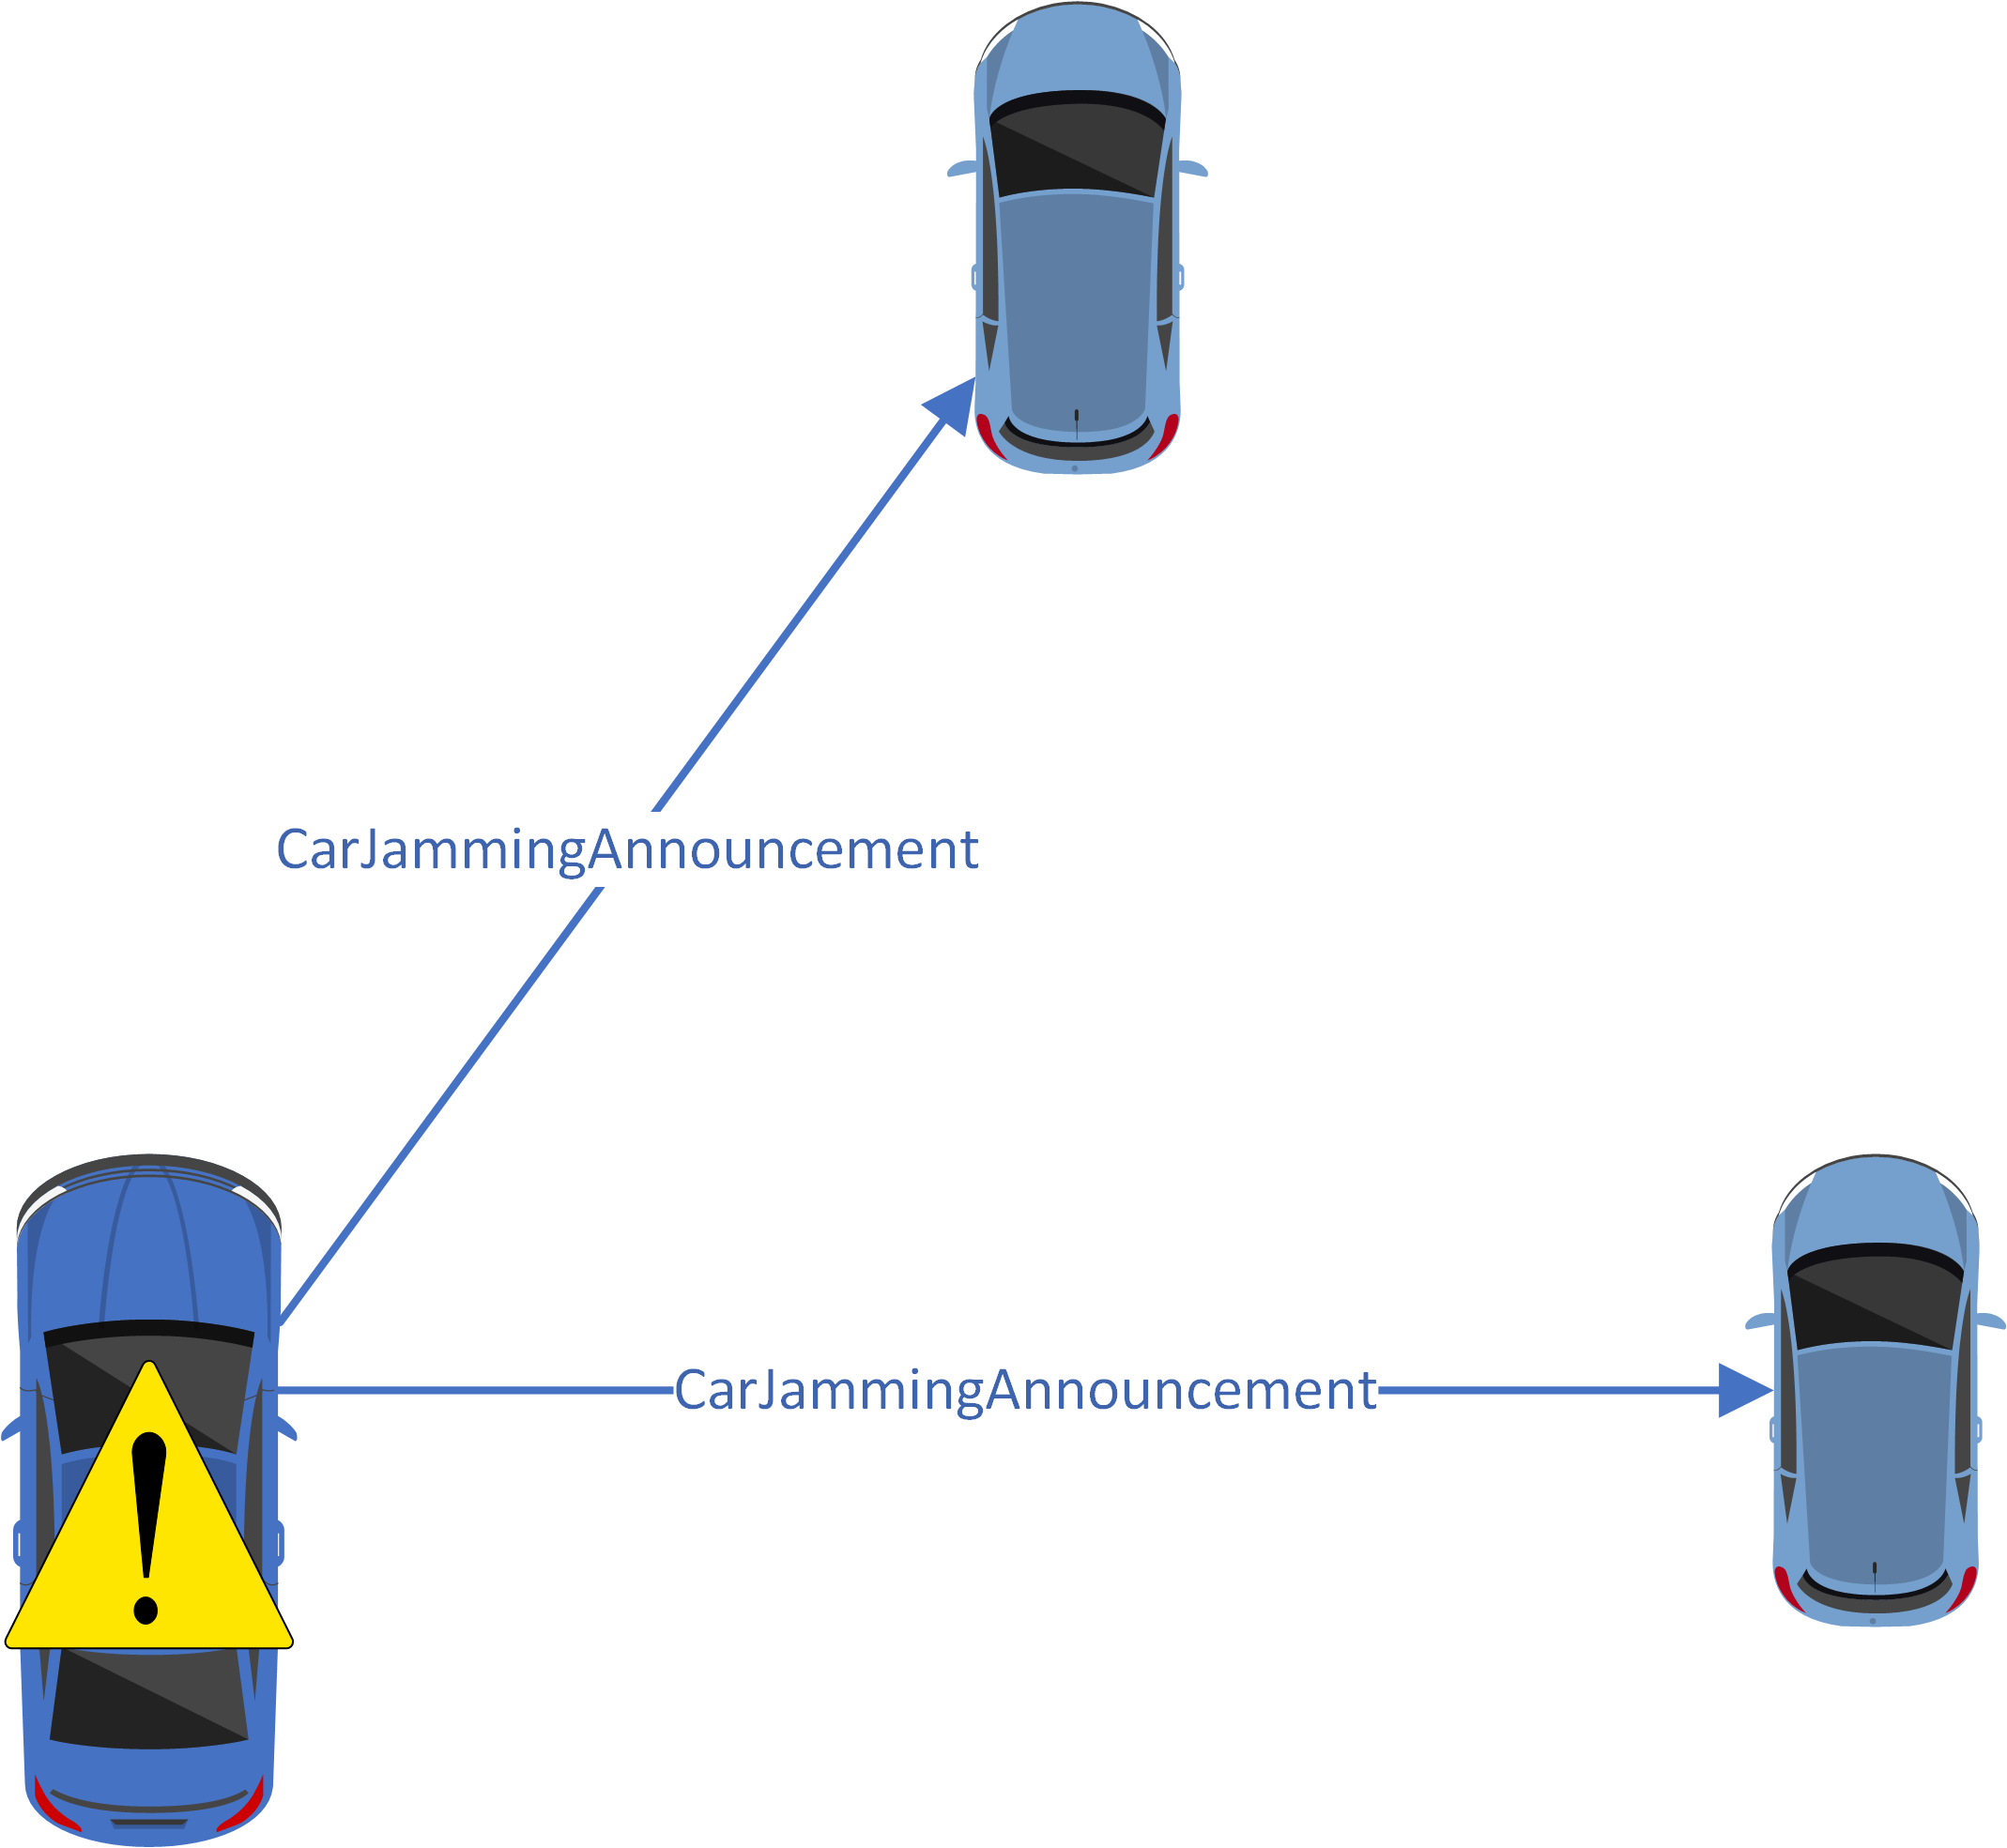
\includegraphics[clip,width=0.5\columnwidth]{figures/Protocol1.png}}
	\subfloat[Step 2]{\label{fig:protocol2}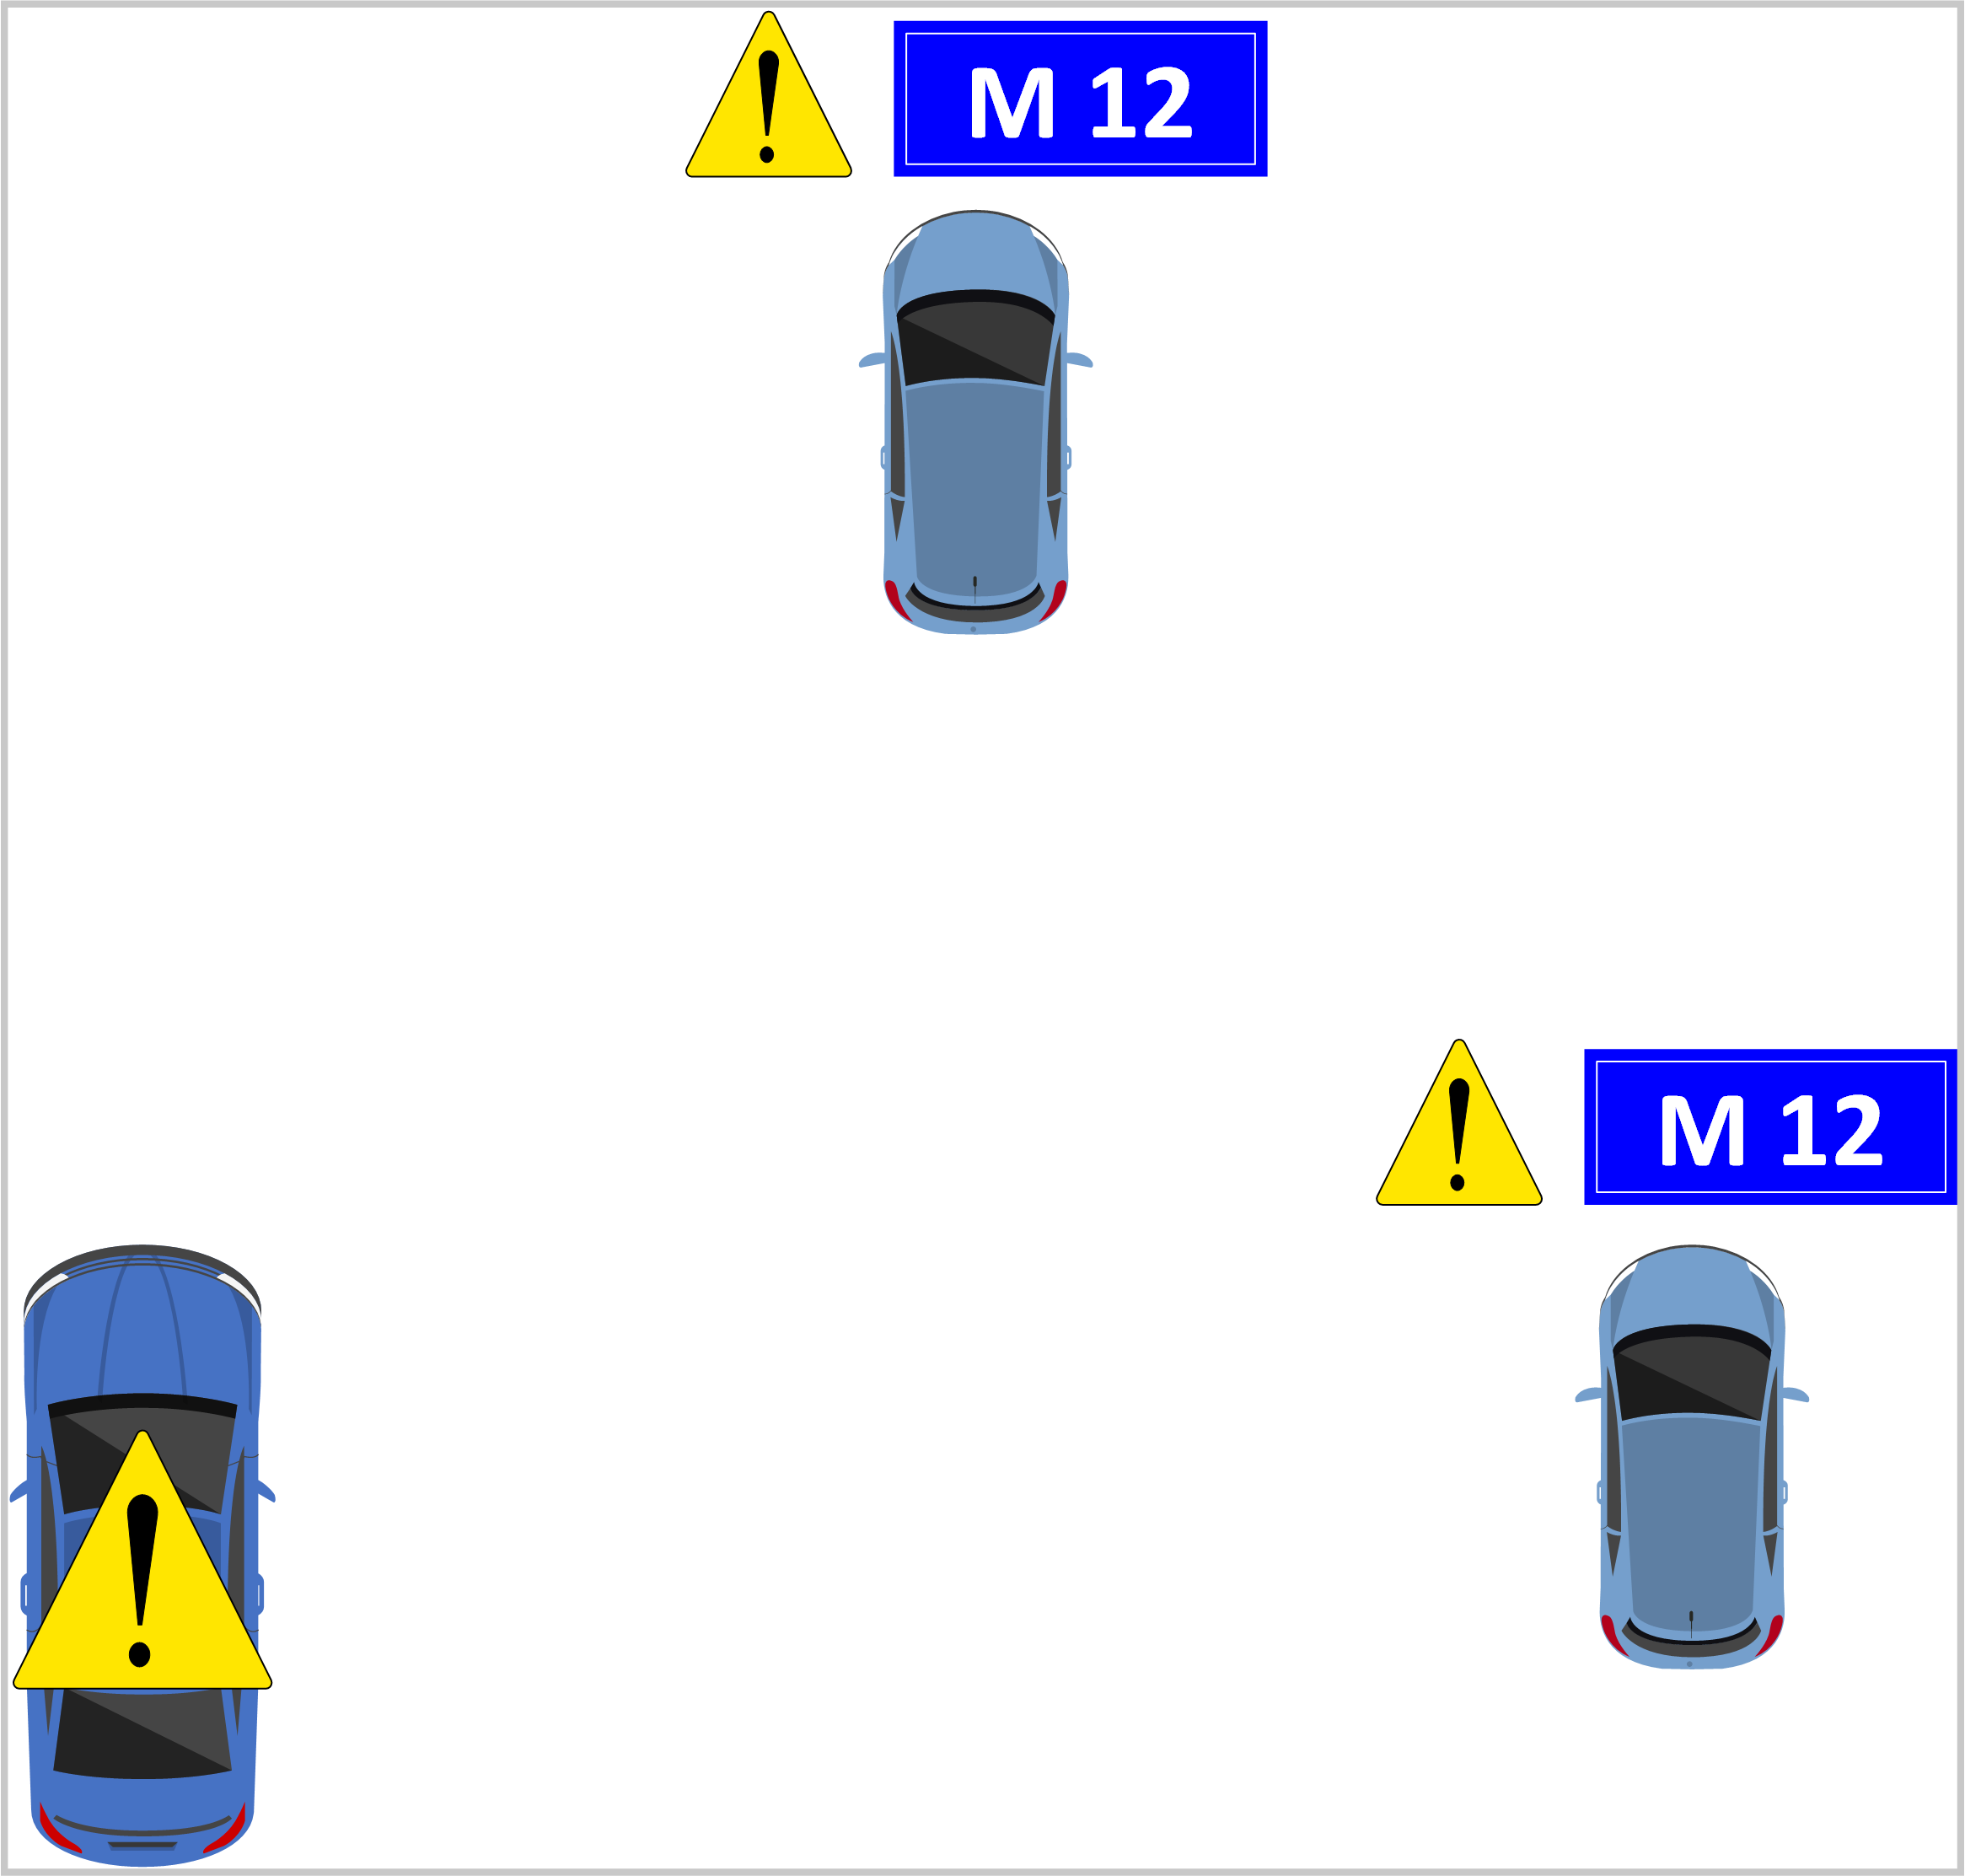
\includegraphics[clip,width=0.5\columnwidth]{figures/Protocol2.png}}
	\subfloat[Step 3]{\label{fig:protocol3}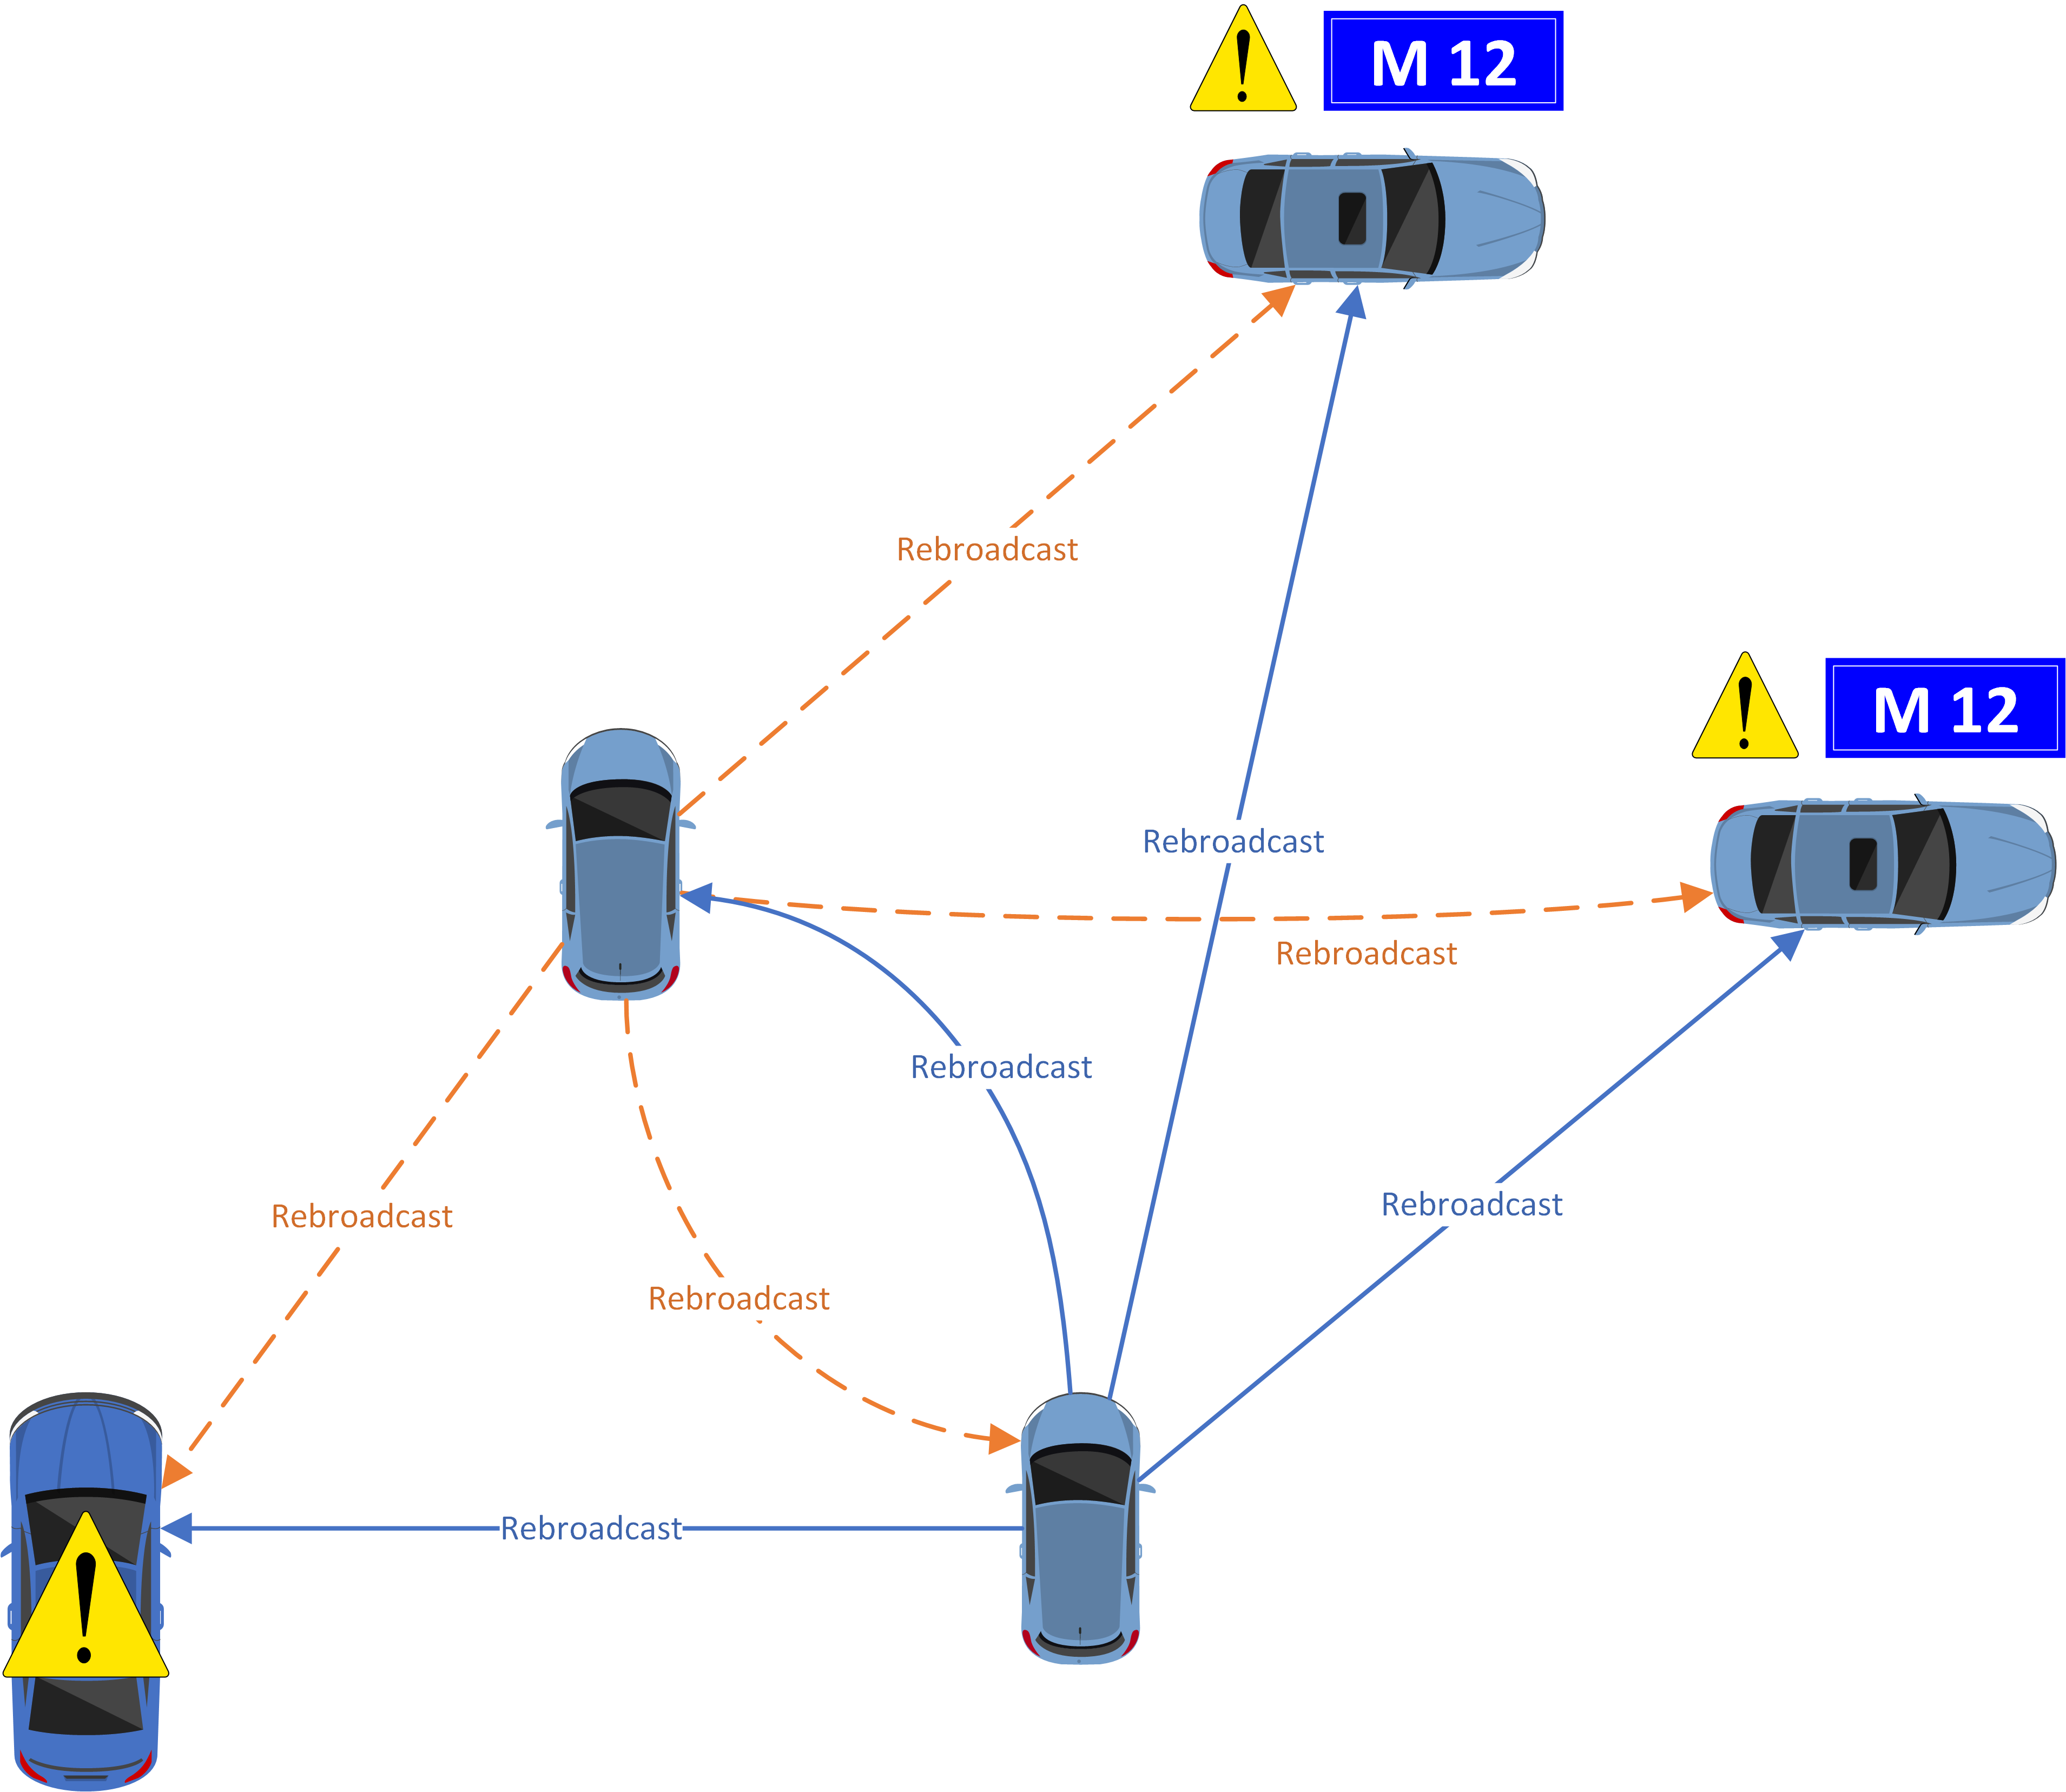
\includegraphics[clip,width=0.5\columnwidth]{figures/Protocol3.png}}
	\caption{Jamming announcement protocol. On step 1 (\cref{fig:protocol1}) the vehicle detects that its speed is zero and broadcasts CarJammingAnnouncement message. The vehicles, who receive the broadcast (\cref{fig:protocol2}), read the road id from the message and adjust their routes in order not to get into the jam. Finally  (\cref{fig:protocol3}), the vehicles rebroadcast the initial message and the receivers perform the same steps. This way the jam announcement propagates through the network. The drones also receive and rebroadcast the announcements in the same manner.}%
	\label{fig:protocol}%
\end{figure}

\section{Pathfinder}

While working on the project, I encountered the need to generate random routes for cars. The Vehicle code in Veins when receiving a message can send a TraCI message to SUMO, which will force the vehicle to re-route, avoiding roads with traffic jams. However, the problem is that in this case, SUMO will re-align the route by the shortest path from the current position of the car to the point to which it was originally going. This led to the fact that the path, which was originally tens of kilometers long, was drastically shortened to hundreds of meters. This caused artifacts in the simulation results. The solution to the problem was the Pathfinder module, which builds random routes for cars, taking into account congestion and a given minimum route length.

There is only one Pathfinder module in the simulation. It stores information about the road structure, taken from the same file that SUMO takes it from. The Pathfinder has methods for constructing random routes. Any vehicle can call these methods if needed and then send the resulting random route to SUMO via TraCI, which will cause the vehicle to follow it.

\chapter{Evaluation}

Now it is time to describe the setup of the experiment, the input and output parameters, and to describe and discuss the results.

\section{Manhatten Grid}



\chapter{Conclusion}

\cleardoublepage

\listofabbreviations
\clearpage

\listoffigures
\clearpage

\listoftables
\clearpage

\printbibliography

\end{document}
